% ! TEX root = ../mechanics.tex

\chapter{低速翼型的气动特性}
\section{翼形的几何尺寸}
机翼是飞行器产生升力的主要部件,一般
都有对称面。平行于机翼对称面所截得的
机翼剖面称为翼剖面(profile)或者翼型(airfoil)。
翼型可以分为两类,一类是圆头尖尾的翼
型,一类是尖头尖尾的翼型。

翼型的尖尾点,称为翼型的{\bfseries 后缘点(trailing edge)}。
在翼型的众轮廓点中,有一点与后缘点的距离最长,
称为翼型的{\bfseries 前缘点(leading edge)}。
连接前缘和后缘的直线段,称为翼型的{\bfseries 弦线(chord line)},
它的长度就是{\bfseries 弦长(chord)}。具体尺寸如下图\ref{fig:profile}。
\begin{figure}[!ht]
	\center
	% ! TEX root = ./Incompressible_Flow_over_Airfoils.tex

\tikzset{every picture/.style={line width=0.75pt}} %set default line width to 0.75pt        

\begin{tikzpicture}[x=0.75pt,y=0.75pt,yscale=-1,xscale=1]
%uncomment if require: \path (0,300); %set diagram left start at 0, and has height of 300

%Straight Lines [id:da022349355429663653] 
\draw [color={rgb, 255:red, 208; green, 2; blue, 27 }  ,draw opacity=1 ]   (150,170) -- (600.91,170.01) ;
\draw [shift={(602.91,170.01)}, rotate = 180] [color={rgb, 255:red, 208; green, 2; blue, 27 }  ,draw opacity=1 ][line width=0.75]    (10.93,-3.29) .. controls (6.95,-1.4) and (3.31,-0.3) .. (0,0) .. controls (3.31,0.3) and (6.95,1.4) .. (10.93,3.29)   ;
%Straight Lines [id:da7882491413488364] 
\draw [color={rgb, 255:red, 208; green, 2; blue, 27 }  ,draw opacity=1 ]   (150,170) -- (150,42) ;
\draw [shift={(150,40)}, rotate = 90] [color={rgb, 255:red, 208; green, 2; blue, 27 }  ,draw opacity=1 ][line width=0.75]    (10.93,-3.29) .. controls (6.95,-1.4) and (3.31,-0.3) .. (0,0) .. controls (3.31,0.3) and (6.95,1.4) .. (10.93,3.29)   ;
%Curve Lines [id:da18776453277648453] 
\draw [color={rgb, 255:red, 74; green, 144; blue, 226 }  ,draw opacity=1 ]   (150,170) .. controls (159.84,99.08) and (455.18,155.08) .. (500,170) ;
%Curve Lines [id:da9694351978719664] 
\draw [color={rgb, 255:red, 74; green, 144; blue, 226 }  ,draw opacity=1 ]   (150,170) .. controls (154.51,192.41) and (437.18,183.08) .. (500,170) ;
%Curve Lines [id:da820196213480765] 
\draw [color={rgb, 255:red, 245; green, 166; blue, 35 }  ,draw opacity=1 ] [dash pattern={on 3.75pt off 3pt on 7.5pt off 1.5pt}]  (150,170) .. controls (192.51,134.41) and (440.51,163.08) .. (500,170) ;
%Straight Lines [id:da36074277196552496] 
\draw    (260,170) -- (260.29,137.81) ;
\draw [shift={(260.31,134.81)}, rotate = 90.51] [fill={rgb, 255:red, 0; green, 0; blue, 0 }  ][line width=0.08]  [draw opacity=0] (8.93,-4.29) -- (0,0) -- (8.93,4.29) -- cycle    ;
%Straight Lines [id:da22940087192646375] 
\draw    (260,170) -- (259.93,181.01) ;
\draw [shift={(259.91,184.01)}, rotate = 270.36] [fill={rgb, 255:red, 0; green, 0; blue, 0 }  ][line width=0.08]  [draw opacity=0] (8.93,-4.29) -- (0,0) -- (8.93,4.29) -- cycle    ;
%Straight Lines [id:da2109846101663837] 
\draw    (260,110) -- (260.31,134.81) ;
%Straight Lines [id:da7789073375096773] 
\draw [line width=0.75]  [dash pattern={on 4.5pt off 4.5pt}]  (132.71,156.41) -- (158.71,162.81) ;
%Straight Lines [id:da4798242817144138] 
\draw    (210,110) -- (258,110) ;
\draw [shift={(260,110)}, rotate = 180] [color={rgb, 255:red, 0; green, 0; blue, 0 }  ][line width=0.75]    (10.93,-3.29) .. controls (6.95,-1.4) and (3.31,-0.3) .. (0,0) .. controls (3.31,0.3) and (6.95,1.4) .. (10.93,3.29)   ;
%Straight Lines [id:da25149340434699075] 
\draw    (210,110) -- (152,110) ;
\draw [shift={(150,110)}, rotate = 360] [color={rgb, 255:red, 0; green, 0; blue, 0 }  ][line width=0.75]    (10.93,-3.29) .. controls (6.95,-1.4) and (3.31,-0.3) .. (0,0) .. controls (3.31,0.3) and (6.95,1.4) .. (10.93,3.29)   ;
%Shape: Circle [id:dp3506292535071094] 
\draw   (150,168.21) .. controls (150,163.67) and (153.67,160) .. (158.21,160) .. controls (162.74,160) and (166.41,163.67) .. (166.41,168.21) .. controls (166.41,172.74) and (162.74,176.41) .. (158.21,176.41) .. controls (153.67,176.41) and (150,172.74) .. (150,168.21) -- cycle ;
%Straight Lines [id:da5413175459804522] 
\draw    (158.21,160) -- (160,170) ;
%Straight Lines [id:da9376674515370762] 
\draw    (310,170) -- (340,200) ;
%Straight Lines [id:da6340913699735564] 
\draw    (260,110) -- (260,100) ;
%Straight Lines [id:da3532135358711779] 
\draw    (270.18,121.75) -- (270.18,142.08) -- (270.18,148.75) ;
\draw [shift={(270.18,151.75)}, rotate = 270] [fill={rgb, 255:red, 0; green, 0; blue, 0 }  ][line width=0.08]  [draw opacity=0] (8.93,-4.29) -- (0,0) -- (8.93,4.29) -- cycle    ;
%Straight Lines [id:da7613828801935856] 
\draw    (270,230) -- (270,173) ;
\draw [shift={(270,170)}, rotate = 90] [fill={rgb, 255:red, 0; green, 0; blue, 0 }  ][line width=0.08]  [draw opacity=0] (8.93,-4.29) -- (0,0) -- (8.93,4.29) -- cycle    ;
%Straight Lines [id:da7363278325234399] 
\draw    (270.18,151.75) -- (270,170) ;
%Straight Lines [id:da0010463214401204013] 
\draw [color={rgb, 255:red, 208; green, 2; blue, 27 }  ,draw opacity=1 ]   (150,170) -- (150,230) ;
%Straight Lines [id:da4725215059330874] 
\draw    (220,200) -- (268,200) ;
\draw [shift={(270,200)}, rotate = 180] [color={rgb, 255:red, 0; green, 0; blue, 0 }  ][line width=0.75]    (10.93,-3.29) .. controls (6.95,-1.4) and (3.31,-0.3) .. (0,0) .. controls (3.31,0.3) and (6.95,1.4) .. (10.93,3.29)   ;
%Straight Lines [id:da6920060964598573] 
\draw    (220,200) -- (152,200) ;
\draw [shift={(150,200)}, rotate = 360] [color={rgb, 255:red, 0; green, 0; blue, 0 }  ][line width=0.75]    (10.93,-3.29) .. controls (6.95,-1.4) and (3.31,-0.3) .. (0,0) .. controls (3.31,0.3) and (6.95,1.4) .. (10.93,3.29)   ;
%Straight Lines [id:da09424509696888994] 
\draw    (477.71,162.01) -- (530.11,180.41) ;
%Straight Lines [id:da767151624060739] 
\draw    (530.11,160.81) -- (485.71,173.21) ;
%Curve Lines [id:da5931692766067793] 
\draw    (516.51,164.41) .. controls (523.71,165.21) and (522.51,174.41) .. (517.31,176.41) ;

% Text Node
\draw (114,162) node [anchor=north west][inner sep=0.75pt]  [color={rgb, 255:red, 65; green, 117; blue, 5 }  ,opacity=1 ] [align=left] { 前缘};
% Text Node
\draw (113,141.4) node [anchor=north west][inner sep=0.75pt]  [color={rgb, 255:red, 126; green, 211; blue, 33 }  ,opacity=1 ]  {$r_{L}$};
% Text Node
\draw (194,91.4) node [anchor=north west][inner sep=0.75pt]  [color={rgb, 255:red, 126; green, 211; blue, 33 }  ,opacity=1 ]  {$x_{t}$};
% Text Node
\draw (191,182.4) node [anchor=north west][inner sep=0.75pt]  [color={rgb, 255:red, 126; green, 211; blue, 33 }  ,opacity=1 ]  {$x_{c}$};
% Text Node
\draw (248,153.4) node [anchor=north west][inner sep=0.75pt]  [color={rgb, 255:red, 126; green, 211; blue, 33 }  ,opacity=1 ]  {$t$};
% Text Node
\draw (276.27,154.5) node [anchor=north west][inner sep=0.75pt]  [color={rgb, 255:red, 126; green, 211; blue, 33 }  ,opacity=1 ]  {$y_{\mathrm{cmax}}$};
% Text Node
\draw (318.4,157) node [anchor=north west][inner sep=0.75pt]  [color={rgb, 255:red, 126; green, 211; blue, 33 }  ,opacity=1 ]  {$c$};
% Text Node
\draw (328,202) node [anchor=north west][inner sep=0.75pt]  [color={rgb, 255:red, 65; green, 117; blue, 5 }  ,opacity=1 ] [align=left] {弦长};
% Text Node
\draw (478,182) node [anchor=north west][inner sep=0.75pt]  [color={rgb, 255:red, 65; green, 117; blue, 5 }  ,opacity=1 ] [align=left] {后缘};
% Text Node
\draw (423,132.4) node [anchor=north west][inner sep=0.75pt]  [color={rgb, 255:red, 126; green, 211; blue, 33 }  ,opacity=1 ]  {$y_{上}(x)$};
% Text Node
\draw (399,183.4) node [anchor=north west][inner sep=0.75pt]  [color={rgb, 255:red, 126; green, 211; blue, 33 }  ,opacity=1 ]  {$y_{下}(x)$};
% Text Node
\draw (536.71,146.01) node [anchor=north west][inner sep=0.75pt]  [color={rgb, 255:red, 65; green, 117; blue, 5 }  ,opacity=1 ] [align=left] {后缘角};
% Text Node
\draw (579.11,170.01) node [anchor=north west][inner sep=0.75pt]  [color={rgb, 255:red, 208; green, 2; blue, 27 }  ,opacity=1 ]  {$x$};
% Text Node
\draw (136.4,44) node [anchor=north west][inner sep=0.75pt]  [color={rgb, 255:red, 208; green, 2; blue, 27 }  ,opacity=1 ]  {$y$};
% Text Node
\draw (512,177) node [anchor=north west][inner sep=0.75pt]  [color={rgb, 255:red, 126; green, 211; blue, 33 }  ,opacity=1 ]  {$\tau $};

\end{tikzpicture}

	\caption{翼型的几何参数定义}
	\label{fig:profile}
\end{figure}
如图\ref{fig:profile}所示,以前缘点为坐标原点,沿弦线建立
$x$轴,垂直弦线向上建立$y$轴,这样的坐标系称为{\bfseries 体坐标系}。
在体坐标系中,弦向的无量纲坐标是$\overline{x}=\frac{x}{c}$。翼型
的上表面和下表面的无量纲坐标分别是
\begin{equation*}
	\begin{cases}
		\overline{y}_上(\overline{x}) & =\frac{y_上(\overline{x})}{c} \\
		\overline{y}_下(\overline{x}) & =\frac{y_下(\overline{x})}{c} \\
	\end{cases}
\end{equation*}

翼型上下表面平行于$y$轴的连线的中点连成的曲线,称为翼型的
{\bfseries 中弧线(mean camber line)}。中弧线可以用来描述
翼型的弯曲程度。中弧线的无量纲坐标$\overline{y}_c(\overline{x})$称为
弯度分布函数,其最大值称为{\bfseries 相对弯度}$\overline{f}=\overline{y}_{cmax}$,
其坐在的弦向位置记为$\overline{x}_c$。
\begin{note}
	如果中弧线是一条直线,这个翼型必为对称翼型。
\end{note}
\begin{notice}
	关于中弧线的解释原文如下:

	The mean camber line is the
	locus of points halfway between the upper and lower surfaces as measured perpendicular
	to the mean camber line itself。
\end{notice}
中弧线的起点和终点分别是前缘点和后缘点。
{\bfseries 厚度(thickness)}是翼型上下表面的距离,
这个距离垂直于弦长。翼型在前缘点附近的形状通常是一段
圆弧,这个圆弧的半径近似是$0.02c$。机翼的气动力和气动
力矩在{\color{titleblue}\ref{气动力和气动力矩}}节已经
讨论,请往回看。

这里讨论对于机翼的属性都是对于无限长的翼型来说的,即
在翼展方向翼型的截面形状不变。

\begin{figure}[!ht]
	\centering
	% ! TEX root = ./Incompressible_Flow_over_Airfoils.tex
\tikzset{every picture/.style={line width=0.75pt}} %set default line width to 0.75pt        

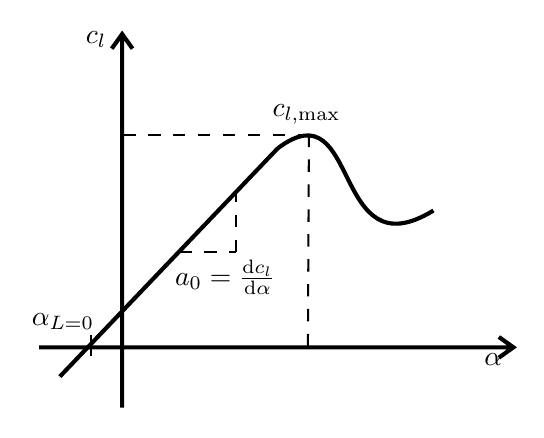
\begin{tikzpicture}[x=0.75pt,y=0.75pt,yscale=-1,xscale=1]
%uncomment if require: \path (0,300); %set diagram left start at 0, and has height of 300

%Shape: Axis 2D [id:dp7499793159263701] 
\draw [line width=1.5]  (200,200.91) -- (428.51,200.91)(240.01,50) -- (240.01,230) (421.51,195.91) -- (428.51,200.91) -- (421.51,205.91) (235.01,57) -- (240.01,50) -- (245.01,57)  ;
%Straight Lines [id:da6818952166992882] 
\draw [line width=1.5]    (315,105) -- (210,215) ;
%Curve Lines [id:da1326114333246986] 
\draw [line width=1.5]    (315,105) .. controls (355,75) and (340.51,165.41) .. (390,135) ;
%Straight Lines [id:da5229353245143065] 
\draw  [dash pattern={on 4.5pt off 4.5pt}]  (240.51,98.41) -- (330.01,98.41) ;
%Straight Lines [id:da4476710750224884] 
\draw  [dash pattern={on 4.5pt off 4.5pt}]  (330.01,98.41) -- (329.51,200.91) ;
%Straight Lines [id:da9636430686615973] 
\draw  [dash pattern={on 4.5pt off 4.5pt}]  (295,125) -- (295,155) ;
%Straight Lines [id:da07371078021099309] 
\draw  [dash pattern={on 4.5pt off 4.5pt}]  (267.51,155) -- (295,155) ;
%Straight Lines [id:da6656415726077622] 
\draw    (225,195) -- (225,205) ;

% Text Node
\draw (221,47.4) node [anchor=north west][inner sep=0.75pt]    {$c_{l}$};
% Text Node
\draw (413,202.4) node [anchor=north west][inner sep=0.75pt]    {$\alpha $};
% Text Node
\draw (195,183) node [anchor=north west][inner sep=0.75pt]    {$\alpha _{L=0}$};
% Text Node
\draw (311,82.4) node [anchor=north west][inner sep=0.75pt]    {$c_{l,\max}$};
% Text Node
\draw (264,157.4) node [anchor=north west][inner sep=0.75pt]    {$a_0=\frac{\mathrm{d}c_l}{\mathrm{d}\alpha}$};


\end{tikzpicture}

	\caption{攻角升力系数曲线}
	\label{fig:angle_of_attack}
\end{figure}

典型的升力系数和攻角之间的变化关系如图\ref{fig:angle_of_attack}所示。
在小攻角和中等攻角的情况下,升力系数随攻角线性变化,这条直线的斜率
记作$a_0$,称为{\bfseries 升力曲线斜率(lift slope)}。在这个区域,空气
从平滑的沿着机翼表面的大部分地方流过。如下图\ref{fig:separate}中左图所示。
\begin{figure}[!ht]
	\centering
	% ! TEX root = ./Incompressible_Flow_over_Airfoils.tex
\tikzset{every picture/.style={line width=0.75pt}} %set default line width to 0.75pt        

\begin{tikzpicture}[x=0.75pt,y=0.75pt,yscale=-1,xscale=1]
%uncomment if require: \path (0,300); %set diagram left start at 0, and has height of 300

%Curve Lines [id:da02066410406444219] 
\draw    (100,121) .. controls (101.51,78.41) and (209.51,108.41) .. (240,120) ;
%Curve Lines [id:da2219924451238391] 
\draw    (380,121) .. controls (381.51,78.41) and (489.51,108.41) .. (520,120) ;
%Curve Lines [id:da14090609932613707] 
\draw    (100,121) .. controls (95.51,131.41) and (187.51,133.41) .. (240,120) ;
%Curve Lines [id:da27960053041213895] 
\draw    (380,121) .. controls (375.51,131.41) and (467.51,133.41) .. (520,120) ;
%Curve Lines [id:da6913211374271631] 
\draw    (80,120) .. controls (106.51,75.41) and (182.51,86.41) .. (240,110) ;
%Curve Lines [id:da7622723644251566] 
\draw    (10,130) .. controls (22.51,129.41) and (59.51,141.41) .. (80,120) ;
%Curve Lines [id:da9760332704223047] 
\draw    (10,150) .. controls (50.51,146.41) and (60,151) .. (100,121) ;
%Curve Lines [id:da5482952107644146] 
\draw    (100,140) .. controls (124.51,140.41) and (190.51,142.41) .. (240,130) ;
%Curve Lines [id:da5631950688908602] 
\draw    (10,170) .. controls (48.51,161.41) and (84.51,139.41) .. (100,140) ;
%Curve Lines [id:da7172273345993287] 
\draw    (360,100) .. controls (395.51,65.41) and (464.51,48.41) .. (520,70) ;
%Curve Lines [id:da6932200849907699] 
\draw    (300,120) .. controls (307.51,117.41) and (327.51,126.41) .. (360,100) ;
%Curve Lines [id:da20447554639464416] 
\draw    (360,130) .. controls (393.51,145.41) and (479.51,143.41) .. (520,130) ;
%Curve Lines [id:da7880084900812823] 
\draw    (300,140) .. controls (309.51,141.41) and (342.51,121.41) .. (360,130) ;
%Curve Lines [id:da0023191113925786766] 
\draw    (470,80) .. controls (462.73,110.47) and (515.2,91.63) .. (492.34,71.84) ;
\draw [shift={(490,70)}, rotate = 35.61] [fill={rgb, 255:red, 0; green, 0; blue, 0 }  ][line width=0.08]  [draw opacity=0] (8.93,-4.29) -- (0,0) -- (8.93,4.29) -- cycle    ;
%Straight Lines [id:da8089051209711549] 
\draw    (150,90) -- (157,90) ;
\draw [shift={(160,90)}, rotate = 180] [fill={rgb, 255:red, 0; green, 0; blue, 0 }  ][line width=0.08]  [draw opacity=0] (8.93,-4.29) -- (0,0) -- (8.93,4.29) -- cycle    ;
%Straight Lines [id:da08051498630628573] 
\draw    (140,140) -- (147,140) ;
\draw [shift={(150,140)}, rotate = 180] [fill={rgb, 255:red, 0; green, 0; blue, 0 }  ][line width=0.08]  [draw opacity=0] (8.93,-4.29) -- (0,0) -- (8.93,4.29) -- cycle    ;
%Straight Lines [id:da1179192395045412] 
\draw    (460,60) -- (467,60) ;
\draw [shift={(470,60)}, rotate = 180] [fill={rgb, 255:red, 0; green, 0; blue, 0 }  ][line width=0.08]  [draw opacity=0] (8.93,-4.29) -- (0,0) -- (8.93,4.29) -- cycle    ;
%Straight Lines [id:da7900053116720815] 
\draw    (440,140) -- (447,140) ;
\draw [shift={(450,140)}, rotate = 180] [fill={rgb, 255:red, 0; green, 0; blue, 0 }  ][line width=0.08]  [draw opacity=0] (8.93,-4.29) -- (0,0) -- (8.93,4.29) -- cycle    ;
%Straight Lines [id:da6440041036552087] 
\draw    (380,50) -- (448.16,79.21) ;
\draw [shift={(450,80)}, rotate = 203.2] [color={rgb, 255:red, 0; green, 0; blue, 0 }  ][line width=0.75]    (10.93,-3.29) .. controls (6.95,-1.4) and (3.31,-0.3) .. (0,0) .. controls (3.31,0.3) and (6.95,1.4) .. (10.93,3.29)   ;

% Text Node
\draw (122,152) node [anchor=north west][inner sep=0.75pt]   [align=left] {小攻角时气流未分离};
% Text Node
\draw (417,151) node [anchor=north west][inner sep=0.75pt]   [align=left] {大攻角下气流分离};
% Text Node
\draw (347,32) node [anchor=north west][inner sep=0.75pt]   [align=left] {分离区域};
% Text Node
\draw (540,112) node [anchor=north west][inner sep=0.75pt]   [align=left] {dead air};


\end{tikzpicture}

	\caption{攻角大小不同时气流流过机翼的流场}
	\label{fig:separate}
\end{figure}
然而,当攻角逐渐变大到一定值时,气流有从翼型上表面分离的趋势,在
机翼后面产生一片“死区空气”(dead air),如图\ref{fig:separate}右图所示。
在气流分离的区域,流动时再循环的。并且有部分流动是与自由来流的方向相
反的,这就是{\bfseries 逆流(reversed flow)}。流动分离主要是因为流体的
粘性效应。
在大攻角下流动分离引起的后果就是{\color{noteorange}升力急剧
减小,阻力急剧增加},这种情况就叫做{\bfseries 失速(stalled)}。

\begin{notice}
	关于流体分离的原文:

	This separated flow is due to
	viscous effects。
\end{notice}
在失速之前,$c_l$的最大值记作$c_{l,\max}$。这是衡量一款翼型的重要指标,
因为它决定了飞机发生失速时的速度。

为了安全起见,把$c_{l \max}$对应的飞行迎角定义为失速迎角,
而不是飞机失速时实际稍高的极限迎角。
\begin{notice}
	$c_{l,\max}$越大,失速速度就越小。
\end{notice}
回到图\ref{fig:angle_of_attack}中,$c_l$随着攻角的增大线性增加,
直到流动分离开始产生影响。然后,曲线开始变成非线性的,$c_l$达到
最大值,最终机翼发生失速。在曲线的另一端,在$\alpha=0$时,升力
是有限的。事实上,只有当飞机低头使得攻角是负的时候,升力才会减小到0。
当升力等于0时的攻角大小叫作{\bfseries 零升攻角(zero-lift angle of attack)},
记作$\alpha_{L=0}$。
\begin{notice}
	对于对称翼型,$\alpha_{L=0}=0$。但是对于大部分有着正弯度的翼型来说,
	$\alpha_{L=0}$是一个负值,一般是$-2$或$-3^{\circ}$的数量级。
\end{notice}

实验表明,升力曲线的斜率不受雷诺数影响,但是$c_{l,\max}$取决于
雷诺数。
\begin{notice}
	因为$c_{l,\max}$被粘性控制,并且雷诺数是一个相似参数,
	它决定了流动中惯性力和粘性力的比值。
\end{notice}

翼型的气动力矩是攻角的函数,但是在翼型上存在一个点,使得气动
力矩的大小和攻角无关,这个点叫做{\bfseries 空气动力中心(aerodynamic center)}。
这个点一般位于距机翼前缘$\frac{c}{4}$的位置。
\begin{example}
	给定翼型为NACA 2412,弦长是$0.64$m,在标准海平面上飞行,自由
	来流的速度是$70$m/s,单位翼展上的升力是$1254$N/m。计算飞行迎角
	和单位翼展上的阻力大小。


	在标准海平面上,$\rho=1.23\text{Kg/m}^3$:
	\[
		q_\infty =\frac{1}{2}\rho_\infty V_\infty ^2 =\frac{1}{2}\times 1.23\times 70^2=3013.5
		\text{N/m}^2
	\]
	\[
		c_l=\frac{L}{q_\infty S}=\frac{L}{q_\infty c}=\frac{1254}{3013.3\times 0.64}=0.65
	\]
	对于$c_l=0.65$,查升力曲线图,得到$\alpha=4^\circ$。

	标准海平面上,$\mu=1.789\times 10^{-5}\text{Kg/m$\cdot$ s}$:
	\[
		\mathrm{Re}=\frac{\rho_\infty V_\infty c }{\mu_\infty}=\frac{14.23\times 70\times 0.64}{1.789\times 10^{-5}}
		=3.08\times 10^6
	\]
	查阻力曲线图,得到$c_d=0.0068$,因此
	\[
		D=q_\infty S c_d=q_\infty c c_d=3013.5\times 0.64\times 0.0068=13.1\text{N/m}
	\]
\end{example}
\begin{example}
	对于NACA 2412翼型,计算并比较攻角分别在$0^\circ$,$4^\circ$,$8^\circ$,$12^\circ$
	时的升阻比,雷诺数是$3.1\times 10^6$。

	查升力曲线图和阻力曲线图得到下表

	\centering
	\begin{tabular}{llll}
		\toprule
		$\alpha$ & $c_l$ & $c_d$  & $c_l /c_d$ \\
		\midrule
		0        & 0.25  & 0.0065 & 38.5       \\
		4        & 0.65  & 0.0070 & 93         \\
		8        & 1.08  & 0.0112 & 96         \\
		12       & 1.44  & 0.017  & 85         \\
		\bottomrule
	\end{tabular}
\end{example}

从上面例题可以看出,随着攻角增大,升阻比先增大,
达到一个最大值,然后减小。升阻比的最大值是翼型
性能的一个重要参数。它能直接表明翼型的效率。
{\color{noteorange}升阻比越大,翼型的效率就越高}。
由于飞机其他部分的阻力,实际飞机的升阻比一般在10到
20这样的量级。

\section{用于低速流动下的机翼的理论解法:面涡}
想象一根直线垂直于纸面,通过一个点$O$,并且向
纸面的里面和外面无限延伸。这条直线就是强度为
$\Gamma$的{\bfseries 涡旋线(vortex filament)}。
通过这根涡旋线在任意垂直于这个涡旋线的平面上
诱导出的流场和强度为$\Gamma$的点涡诱导出的流
场是一样的。事实上,可以将涡旋线看成是无数点
涡组成的。

对于一个涡流场,考虑和面源相似的情况。想象
无数根涡旋线紧挨着,这些涡旋线的强度又是无穷小。
这些涡旋线就形成了一个{\bfseries 面涡(vortex sheet)}。
顺着这些涡旋线看去,面涡就会变成如图\ref{fig:vortex sheet}
所示的场景。
\begin{figure}[!ht]
  \centering
  % ! TEX root = ./Incompressible_Flow_over_Airfoils.tex

\tikzset{every picture/.style={line width=0.75pt}} %set default line width to 0.75pt        

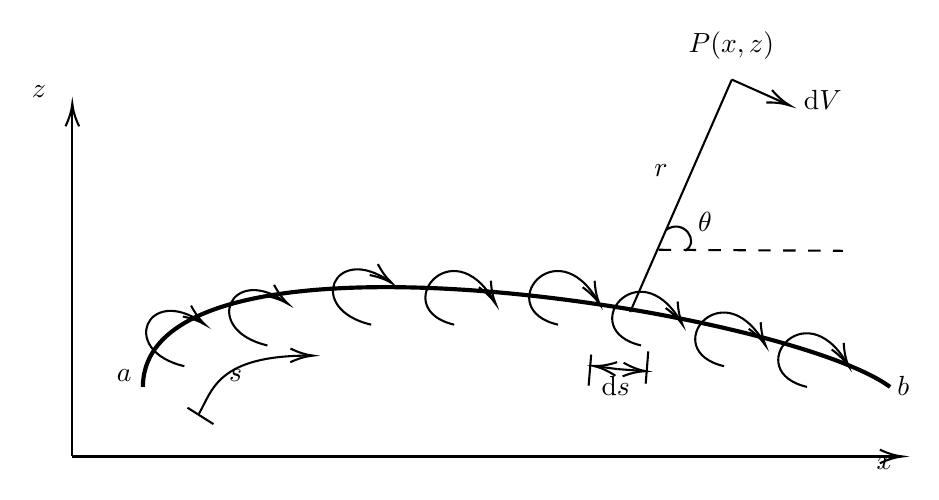
\begin{tikzpicture}[x=0.75pt,y=0.75pt,yscale=-1,xscale=1]
%uncomment if require: \path (0,285); %set diagram left start at 0, and has height of 285

%Curve Lines [id:da8763652678817189] 
\draw [line width=1.5]    (104,206.5) .. controls (104.51,119.91) and (414,169.5) .. (464,206.5) ;
%Curve Lines [id:da4750021580535706] 
\draw    (124,196.5) .. controls (92,189.03) and (106.07,156.9) .. (132.77,175.61) ;
\draw [shift={(134,176.5)}, rotate = 216.83] [color={rgb, 255:red, 0; green, 0; blue, 0 }  ][line width=0.75]    (10.93,-3.29) .. controls (6.95,-1.4) and (3.31,-0.3) .. (0,0) .. controls (3.31,0.3) and (6.95,1.4) .. (10.93,3.29)   ;
%Curve Lines [id:da2895808384347458] 
\draw    (164,186.5) .. controls (132,179.03) and (146.07,146.9) .. (172.77,165.61) ;
\draw [shift={(174,166.5)}, rotate = 216.83] [color={rgb, 255:red, 0; green, 0; blue, 0 }  ][line width=0.75]    (10.93,-3.29) .. controls (6.95,-1.4) and (3.31,-0.3) .. (0,0) .. controls (3.31,0.3) and (6.95,1.4) .. (10.93,3.29)   ;
%Curve Lines [id:da7153231460572151] 
\draw    (214,176.5) .. controls (182,169.03) and (196.07,136.9) .. (222.77,155.61) ;
\draw [shift={(224,156.5)}, rotate = 216.83] [color={rgb, 255:red, 0; green, 0; blue, 0 }  ][line width=0.75]    (10.93,-3.29) .. controls (6.95,-1.4) and (3.31,-0.3) .. (0,0) .. controls (3.31,0.3) and (6.95,1.4) .. (10.93,3.29)   ;
%Curve Lines [id:da9877697377632966] 
\draw    (254,176.5) .. controls (222,169.03) and (252.56,130.11) .. (273.07,164.86) ;
\draw [shift={(274,166.5)}, rotate = 241.4] [color={rgb, 255:red, 0; green, 0; blue, 0 }  ][line width=0.75]    (10.93,-3.29) .. controls (6.95,-1.4) and (3.31,-0.3) .. (0,0) .. controls (3.31,0.3) and (6.95,1.4) .. (10.93,3.29)   ;
%Curve Lines [id:da6202187083118886] 
\draw    (304,176.5) .. controls (272,169.03) and (302.56,130.11) .. (323.07,164.86) ;
\draw [shift={(324,166.5)}, rotate = 241.4] [color={rgb, 255:red, 0; green, 0; blue, 0 }  ][line width=0.75]    (10.93,-3.29) .. controls (6.95,-1.4) and (3.31,-0.3) .. (0,0) .. controls (3.31,0.3) and (6.95,1.4) .. (10.93,3.29)   ;
%Curve Lines [id:da8336758488674814] 
\draw    (344,186.5) .. controls (312,179.03) and (342.56,140.11) .. (363.07,174.86) ;
\draw [shift={(364,176.5)}, rotate = 241.4] [color={rgb, 255:red, 0; green, 0; blue, 0 }  ][line width=0.75]    (10.93,-3.29) .. controls (6.95,-1.4) and (3.31,-0.3) .. (0,0) .. controls (3.31,0.3) and (6.95,1.4) .. (10.93,3.29)   ;
%Curve Lines [id:da8897778956265143] 
\draw    (384,196.5) .. controls (352,189.03) and (382.56,150.11) .. (403.07,184.86) ;
\draw [shift={(404,186.5)}, rotate = 241.4] [color={rgb, 255:red, 0; green, 0; blue, 0 }  ][line width=0.75]    (10.93,-3.29) .. controls (6.95,-1.4) and (3.31,-0.3) .. (0,0) .. controls (3.31,0.3) and (6.95,1.4) .. (10.93,3.29)   ;
%Curve Lines [id:da04487167241342771] 
\draw    (424,206.5) .. controls (392,199.03) and (422.56,160.11) .. (443.07,194.86) ;
\draw [shift={(444,196.5)}, rotate = 241.4] [color={rgb, 255:red, 0; green, 0; blue, 0 }  ][line width=0.75]    (10.93,-3.29) .. controls (6.95,-1.4) and (3.31,-0.3) .. (0,0) .. controls (3.31,0.3) and (6.95,1.4) .. (10.93,3.29)   ;
%Straight Lines [id:da5621055060339388] 
\draw    (125.5,216.5) -- (138.01,224.41) ;
%Curve Lines [id:da3596797142445818] 
\draw    (131.01,219.41) .. controls (137.45,208.52) and (139.47,191.26) .. (184.63,191.4) ;
\draw [shift={(186.01,191.41)}, rotate = 180.62] [color={rgb, 255:red, 0; green, 0; blue, 0 }  ][line width=0.75]    (10.93,-3.29) .. controls (6.95,-1.4) and (3.31,-0.3) .. (0,0) .. controls (3.31,0.3) and (6.95,1.4) .. (10.93,3.29)   ;
%Straight Lines [id:da4909959828720716] 
\draw    (347.5,189.41) -- (346.26,204.91) ;
%Straight Lines [id:da5091055511160192] 
\draw    (318.76,205.91) -- (320,190.91) ;
%Straight Lines [id:da5213093595184453] 
\draw    (332.76,197.91) -- (344.27,198.77) ;
\draw [shift={(346.26,198.91)}, rotate = 184.24] [color={rgb, 255:red, 0; green, 0; blue, 0 }  ][line width=0.75]    (10.93,-3.29) .. controls (6.95,-1.4) and (3.31,-0.3) .. (0,0) .. controls (3.31,0.3) and (6.95,1.4) .. (10.93,3.29)   ;
%Straight Lines [id:da04498336011734372] 
\draw    (332.76,197.91) -- (323.24,196.67) ;
\draw [shift={(321.26,196.41)}, rotate = 7.43] [color={rgb, 255:red, 0; green, 0; blue, 0 }  ][line width=0.75]    (10.93,-3.29) .. controls (6.95,-1.4) and (3.31,-0.3) .. (0,0) .. controls (3.31,0.3) and (6.95,1.4) .. (10.93,3.29)   ;
%Straight Lines [id:da31365051851853876] 
\draw    (338.76,170.41) -- (387.76,58.41) ;
%Straight Lines [id:da29570303575193213] 
\draw  [dash pattern={on 4.5pt off 4.5pt}]  (352.5,140.41) -- (368.26,140.5) -- (441.26,140.91) ;
%Curve Lines [id:da3186708293732772] 
\draw    (356,130.91) .. controls (364.26,124.91) and (372.76,136.41) .. (365.26,140.91) ;
%Straight Lines [id:da09450810625839368] 
\draw    (387.76,58.41) -- (413.94,70.1) ;
\draw [shift={(415.76,70.91)}, rotate = 204.06] [color={rgb, 255:red, 0; green, 0; blue, 0 }  ][line width=0.75]    (10.93,-3.29) .. controls (6.95,-1.4) and (3.31,-0.3) .. (0,0) .. controls (3.31,0.3) and (6.95,1.4) .. (10.93,3.29)   ;
%Straight Lines [id:da5222357770732207] 
\draw    (70,240) -- (70,72) ;
\draw [shift={(70,70)}, rotate = 90] [color={rgb, 255:red, 0; green, 0; blue, 0 }  ][line width=0.75]    (10.93,-3.29) .. controls (6.95,-1.4) and (3.31,-0.3) .. (0,0) .. controls (3.31,0.3) and (6.95,1.4) .. (10.93,3.29)   ;
%Straight Lines [id:da5641055148269973] 
\draw    (70,240) -- (468,240) ;
\draw [shift={(470,240)}, rotate = 180] [color={rgb, 255:red, 0; green, 0; blue, 0 }  ][line width=0.75]    (10.93,-3.29) .. controls (6.95,-1.4) and (3.31,-0.3) .. (0,0) .. controls (3.31,0.3) and (6.95,1.4) .. (10.93,3.29)   ;

% Text Node
\draw (90,196.5) node [anchor=north west][inner sep=0.75pt]    {$a$};
% Text Node
\draw (144,196.5) node [anchor=north west][inner sep=0.75pt]    {$s$};
% Text Node
\draw (466,200) node [anchor=north west][inner sep=0.75pt]    {$b$};
% Text Node
\draw (323.5,199.91) node [anchor=north west][inner sep=0.75pt]    {$\mathrm{d}s$};
% Text Node
\draw (349,97.91) node [anchor=north west][inner sep=0.75pt]    {$r$};
% Text Node
\draw (370,120.91) node [anchor=north west][inner sep=0.75pt]    {$\theta $};
% Text Node
\draw (365.5,33.91) node [anchor=north west][inner sep=0.75pt]    {$P(x,z)$};
% Text Node
\draw (421,61.91) node [anchor=north west][inner sep=0.75pt]    {$\mathrm{d}V$};
% Text Node
\draw (49,60) node [anchor=north west][inner sep=0.75pt]    {$z$};
% Text Node
\draw (456,239) node [anchor=north west][inner sep=0.75pt]    {$x$};


\end{tikzpicture}

  \caption{面涡的边缘视角}
  \label{fig:vortex sheet}
\end{figure}
所有的涡旋线都垂直于纸面。设$s$是沿着面涡边缘
视角下的距离坐标。定义$\gamma=\gamma(s)$是
坐标为$s$的单位长度上面涡的强度。因此,对于
无限小长度$\mathrm{d}s$上的面涡强度就是
$\gamma\mathrm{d}s$。面涡的这一小部分
可以看成是强度为$\gamma\mathrm{d}s $的点涡。
现在考虑位于流场中的一个点$P$,和$\mathrm{d}s$的距离
是$r$;坐标是$(x,z)$。强度为$\gamma\mathrm{d}s$的
面涡在$P$点诱导出无穷小的速度$\mathrm{d}V$,即
\[
  \mathrm{d}V=-\frac{\gamma \mathrm{d}s }{2\pi r }
\]
并且方向垂直于$r$。$P$点的诱导速度就是整个面涡从
$a$点到$b$点上式的总和。不同面涡部分在$P$点产生的
速度的叠加必须是矢量叠加的。由于这个,使得处理速度势
就更方便了。通过单元涡$\gamma \mathrm{d}s $在$P$点
诱导出的速度势$\mathrm{d} \Phi$的增量就是
\[
  \mathrm{d}\Phi=-\frac{\gamma \mathrm{d}s }{2\pi}\theta
\]
相应的,从$a$到$b $整个面涡在$P$点的速度势就是
\[
  \Phi(x,z)=- \frac{1}{2\pi}\int _a^b \theta \gamma \mathrm{d}s 
\]
上面这个方程对于薄翼理论的讨论是特别有用的,同时对于涡面元的
数值解法也是特别重要的。

一个点涡的环量$\Gamma$等于这个涡的强度。在图\ref{fig:vortex sheet}
中面涡的环量就是这些涡单元的强度的总和;即
\[
  \Gamma=\int _a^b \gamma \mathrm{d}s 
\]

面源的法向速度分量是不连续的,而速度的切向分量在
面源的上方和下方是一样的。与面源恰恰相反,面涡的切向
速度分量是不连续的,而法向速度分量是连续的。速度的
切向分量的变化大小和面涡的强度是有关系的。考虑一个面涡
如下图\ref{fig:strength_vortex}所示,
\begin{figure}[!ht]
  \centering
  % !TEX root = ./Incompressible_Flow_over_Airfoils.tex

\tikzset{every picture/.style={line width=0.75pt}} %set default line width to 0.75pt        

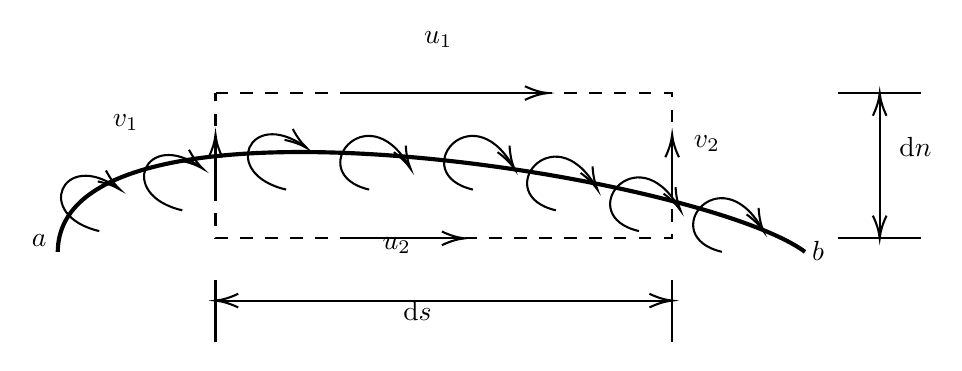
\begin{tikzpicture}[x=0.75pt,y=0.75pt,yscale=-1,xscale=1]
%uncomment if require: \path (0,285); %set diagram left start at 0, and has height of 285

%Curve Lines [id:da8763652678817189] 
\draw [line width=1.5]    (104,206.5) .. controls (104.51,119.91) and (414,169.5) .. (464,206.5) ;
%Curve Lines [id:da4750021580535706] 
\draw    (124,196.5) .. controls (92,189.03) and (106.07,156.9) .. (132.77,175.61) ;
\draw [shift={(134,176.5)}, rotate = 216.83] [color={rgb, 255:red, 0; green, 0; blue, 0 }  ][line width=0.75]    (10.93,-3.29) .. controls (6.95,-1.4) and (3.31,-0.3) .. (0,0) .. controls (3.31,0.3) and (6.95,1.4) .. (10.93,3.29)   ;
%Curve Lines [id:da2895808384347458] 
\draw    (164,186.5) .. controls (132,179.03) and (146.07,146.9) .. (172.77,165.61) ;
\draw [shift={(174,166.5)}, rotate = 216.83] [color={rgb, 255:red, 0; green, 0; blue, 0 }  ][line width=0.75]    (10.93,-3.29) .. controls (6.95,-1.4) and (3.31,-0.3) .. (0,0) .. controls (3.31,0.3) and (6.95,1.4) .. (10.93,3.29)   ;
%Curve Lines [id:da7153231460572151] 
\draw    (214,176.5) .. controls (182,169.03) and (196.07,136.9) .. (222.77,155.61) ;
\draw [shift={(224,156.5)}, rotate = 216.83] [color={rgb, 255:red, 0; green, 0; blue, 0 }  ][line width=0.75]    (10.93,-3.29) .. controls (6.95,-1.4) and (3.31,-0.3) .. (0,0) .. controls (3.31,0.3) and (6.95,1.4) .. (10.93,3.29)   ;
%Curve Lines [id:da9877697377632966] 
\draw    (254,176.5) .. controls (222,169.03) and (252.56,130.11) .. (273.07,164.86) ;
\draw [shift={(274,166.5)}, rotate = 241.4] [color={rgb, 255:red, 0; green, 0; blue, 0 }  ][line width=0.75]    (10.93,-3.29) .. controls (6.95,-1.4) and (3.31,-0.3) .. (0,0) .. controls (3.31,0.3) and (6.95,1.4) .. (10.93,3.29)   ;
%Curve Lines [id:da6202187083118886] 
\draw    (304,176.5) .. controls (272,169.03) and (302.56,130.11) .. (323.07,164.86) ;
\draw [shift={(324,166.5)}, rotate = 241.4] [color={rgb, 255:red, 0; green, 0; blue, 0 }  ][line width=0.75]    (10.93,-3.29) .. controls (6.95,-1.4) and (3.31,-0.3) .. (0,0) .. controls (3.31,0.3) and (6.95,1.4) .. (10.93,3.29)   ;
%Curve Lines [id:da8336758488674814] 
\draw    (344,186.5) .. controls (312,179.03) and (342.56,140.11) .. (363.07,174.86) ;
\draw [shift={(364,176.5)}, rotate = 241.4] [color={rgb, 255:red, 0; green, 0; blue, 0 }  ][line width=0.75]    (10.93,-3.29) .. controls (6.95,-1.4) and (3.31,-0.3) .. (0,0) .. controls (3.31,0.3) and (6.95,1.4) .. (10.93,3.29)   ;
%Curve Lines [id:da8897778956265143] 
\draw    (384,196.5) .. controls (352,189.03) and (382.56,150.11) .. (403.07,184.86) ;
\draw [shift={(404,186.5)}, rotate = 241.4] [color={rgb, 255:red, 0; green, 0; blue, 0 }  ][line width=0.75]    (10.93,-3.29) .. controls (6.95,-1.4) and (3.31,-0.3) .. (0,0) .. controls (3.31,0.3) and (6.95,1.4) .. (10.93,3.29)   ;
%Curve Lines [id:da04487167241342771] 
\draw    (424,206.5) .. controls (392,199.03) and (422.56,160.11) .. (443.07,194.86) ;
\draw [shift={(444,196.5)}, rotate = 241.4] [color={rgb, 255:red, 0; green, 0; blue, 0 }  ][line width=0.75]    (10.93,-3.29) .. controls (6.95,-1.4) and (3.31,-0.3) .. (0,0) .. controls (3.31,0.3) and (6.95,1.4) .. (10.93,3.29)   ;
%Shape: Rectangle [id:dp15963879701718064] 
\draw  [dash pattern={on 4.5pt off 4.5pt}] (180,130) -- (400,130) -- (400,200) -- (180,200) -- cycle ;
%Straight Lines [id:da8026280446997687] 
\draw    (240,130) -- (338,130) ;
\draw [shift={(340,130)}, rotate = 180] [color={rgb, 255:red, 0; green, 0; blue, 0 }  ][line width=0.75]    (10.93,-3.29) .. controls (6.95,-1.4) and (3.31,-0.3) .. (0,0) .. controls (3.31,0.3) and (6.95,1.4) .. (10.93,3.29)   ;
%Straight Lines [id:da3245350317643181] 
\draw    (240,200) -- (298,200) ;
\draw [shift={(300,200)}, rotate = 180] [color={rgb, 255:red, 0; green, 0; blue, 0 }  ][line width=0.75]    (10.93,-3.29) .. controls (6.95,-1.4) and (3.31,-0.3) .. (0,0) .. controls (3.31,0.3) and (6.95,1.4) .. (10.93,3.29)   ;
%Straight Lines [id:da7628086801385121] 
\draw    (180,180) -- (180,152) ;
\draw [shift={(180,150)}, rotate = 90] [color={rgb, 255:red, 0; green, 0; blue, 0 }  ][line width=0.75]    (10.93,-3.29) .. controls (6.95,-1.4) and (3.31,-0.3) .. (0,0) .. controls (3.31,0.3) and (6.95,1.4) .. (10.93,3.29)   ;
%Straight Lines [id:da347003095117139] 
\draw    (400,180) -- (400,152) ;
\draw [shift={(400,150)}, rotate = 90] [color={rgb, 255:red, 0; green, 0; blue, 0 }  ][line width=0.75]    (10.93,-3.29) .. controls (6.95,-1.4) and (3.31,-0.3) .. (0,0) .. controls (3.31,0.3) and (6.95,1.4) .. (10.93,3.29)   ;
%Straight Lines [id:da6243635216764141] 
\draw    (180,220) -- (180,250) ;
%Straight Lines [id:da6817985927803263] 
\draw    (400,220) -- (400,250) ;
%Straight Lines [id:da9105574441608693] 
\draw    (290,230) -- (398,230) ;
\draw [shift={(400,230)}, rotate = 180] [color={rgb, 255:red, 0; green, 0; blue, 0 }  ][line width=0.75]    (10.93,-3.29) .. controls (6.95,-1.4) and (3.31,-0.3) .. (0,0) .. controls (3.31,0.3) and (6.95,1.4) .. (10.93,3.29)   ;
%Straight Lines [id:da7767579818993569] 
\draw    (290,230) -- (182,230) ;
\draw [shift={(180,230)}, rotate = 360] [color={rgb, 255:red, 0; green, 0; blue, 0 }  ][line width=0.75]    (10.93,-3.29) .. controls (6.95,-1.4) and (3.31,-0.3) .. (0,0) .. controls (3.31,0.3) and (6.95,1.4) .. (10.93,3.29)   ;
%Straight Lines [id:da3361994371134467] 
\draw    (480,200) -- (520,200) ;
%Straight Lines [id:da04570162822709278] 
\draw    (480,130) -- (520,130) ;
%Straight Lines [id:da6631521119255424] 
\draw    (500,160) -- (500,198) ;
\draw [shift={(500,200)}, rotate = 270] [color={rgb, 255:red, 0; green, 0; blue, 0 }  ][line width=0.75]    (10.93,-3.29) .. controls (6.95,-1.4) and (3.31,-0.3) .. (0,0) .. controls (3.31,0.3) and (6.95,1.4) .. (10.93,3.29)   ;
%Straight Lines [id:da14321333492030197] 
\draw    (500,160) -- (500,132) ;
\draw [shift={(500,130)}, rotate = 90] [color={rgb, 255:red, 0; green, 0; blue, 0 }  ][line width=0.75]    (10.93,-3.29) .. controls (6.95,-1.4) and (3.31,-0.3) .. (0,0) .. controls (3.31,0.3) and (6.95,1.4) .. (10.93,3.29)   ;

% Text Node
\draw (90,196.5) node [anchor=north west][inner sep=0.75pt]    {$a$};
% Text Node
\draw (466,200) node [anchor=north west][inner sep=0.75pt]    {$b$};
% Text Node
\draw (279,99) node [anchor=north west][inner sep=0.75pt]    {$u_{1}$};
% Text Node
\draw (259,198) node [anchor=north west][inner sep=0.75pt]    {$u_{2}$};
% Text Node
\draw (129,139) node [anchor=north west][inner sep=0.75pt]    {$v_{1}$};
% Text Node
\draw (409,149) node [anchor=north west][inner sep=0.75pt]    {$v_{2}$};
% Text Node
\draw (269,229) node [anchor=north west][inner sep=0.75pt]    {$\mathrm{d}s$};
% Text Node
\draw (508,150) node [anchor=north west][inner sep=0.75pt]    {$\mathrm{d}n$};


\end{tikzpicture}

  \caption{面涡切向分量的跳跃}
  \label{fig:strength_vortex}
\end{figure}
使用一个虚线的矩形框包围一部分面涡,长度是$\mathrm{d}s $。
速度在上下的切向分量分别是$u_1$和$u_2$,左右两边的切向
分量分别是$v_1$和$v_2$,上下两边的距离是$\mathrm{d}n $。
从环量的定义,可以得到这个虚线框的环量是
\[
  \Gamma=-(v_2 \mathrm{d}n -u_1 \mathrm{d}s -v_1 \mathrm{d}n +u_2 \mathrm{d}s)
\]
或
\[
  \Gamma= (u_1-u_2) \mathrm{d}s+(v_1-v_2) \mathrm{d}n
\]
然而,因为包围在虚线路径中的面涡的强度是$\gamma \mathrm{d}s $,于是
\[
  \Gamma =\gamma \mathrm{d}s 
\]
因此
\[
  \gamma \mathrm{d} s =(u_1-u_2 )\mathrm{d}s+(v_1-v_2) \mathrm{d}n
\]
现在让上下表面靠近面涡,即$\mathrm{d}n \rightarrow 0$。在
极限情况下,$u_1$和$u_2$就迅速称为面涡上下表面的切向速度,
上式就可以写成
\[
  \gamma \mathrm{d}s =(u_1-u_2)\mathrm{d}s 
\]
或者
\[
  \gamma =u_1-u_2
\]
这个等式非常重要。它表明了{\bfseries 当地面涡切向速度跳跃的差值
就等于当地面涡的强度}。

面涡的概念是在低速翼型性质分析中的一个工具。考虑在自由来流的速度
为$V_\infty$中的有着任意形状和厚度的翼型,如图\ref{fig:distributing}
\begin{figure}[!ht]
  \centering
  % ! TEX root = ./Incompressible_Flow_over_Airfoils.tex

\tikzset{every picture/.style={line width=0.75pt}} %set default line width to 0.75pt        

\begin{tikzpicture}[x=0.75pt,y=0.75pt,yscale=-1,xscale=1]
%uncomment if require: \path (0,285); %set diagram left start at 0, and has height of 285

%Curve Lines [id:da8763652678817189] 
\draw [line width=1.5]    (180,206.5) .. controls (180.51,119.91) and (490,169.5) .. (540,206.5) ;
%Curve Lines [id:da4750021580535706] 
\draw    (200,196.5) .. controls (168,189.03) and (182.07,156.9) .. (208.77,175.61) ;
\draw [shift={(210,176.5)}, rotate = 216.83] [color={rgb, 255:red, 0; green, 0; blue, 0 }  ][line width=0.75]    (10.93,-3.29) .. controls (6.95,-1.4) and (3.31,-0.3) .. (0,0) .. controls (3.31,0.3) and (6.95,1.4) .. (10.93,3.29)   ;
%Curve Lines [id:da2895808384347458] 
\draw    (240,186.5) .. controls (208,179.03) and (222.07,146.9) .. (248.77,165.61) ;
\draw [shift={(250,166.5)}, rotate = 216.83] [color={rgb, 255:red, 0; green, 0; blue, 0 }  ][line width=0.75]    (10.93,-3.29) .. controls (6.95,-1.4) and (3.31,-0.3) .. (0,0) .. controls (3.31,0.3) and (6.95,1.4) .. (10.93,3.29)   ;
%Curve Lines [id:da7153231460572151] 
\draw    (290,176.5) .. controls (258,169.03) and (272.07,136.9) .. (298.77,155.61) ;
\draw [shift={(300,156.5)}, rotate = 216.83] [color={rgb, 255:red, 0; green, 0; blue, 0 }  ][line width=0.75]    (10.93,-3.29) .. controls (6.95,-1.4) and (3.31,-0.3) .. (0,0) .. controls (3.31,0.3) and (6.95,1.4) .. (10.93,3.29)   ;
%Curve Lines [id:da9877697377632966] 
\draw    (330,176.5) .. controls (298,169.03) and (328.56,130.11) .. (349.07,164.86) ;
\draw [shift={(350,166.5)}, rotate = 241.4] [color={rgb, 255:red, 0; green, 0; blue, 0 }  ][line width=0.75]    (10.93,-3.29) .. controls (6.95,-1.4) and (3.31,-0.3) .. (0,0) .. controls (3.31,0.3) and (6.95,1.4) .. (10.93,3.29)   ;
%Curve Lines [id:da6202187083118886] 
\draw    (380,176.5) .. controls (348,169.03) and (378.56,130.11) .. (399.07,164.86) ;
\draw [shift={(400,166.5)}, rotate = 241.4] [color={rgb, 255:red, 0; green, 0; blue, 0 }  ][line width=0.75]    (10.93,-3.29) .. controls (6.95,-1.4) and (3.31,-0.3) .. (0,0) .. controls (3.31,0.3) and (6.95,1.4) .. (10.93,3.29)   ;
%Curve Lines [id:da8336758488674814] 
\draw    (420,186.5) .. controls (388,179.03) and (418.56,140.11) .. (439.07,174.86) ;
\draw [shift={(440,176.5)}, rotate = 241.4] [color={rgb, 255:red, 0; green, 0; blue, 0 }  ][line width=0.75]    (10.93,-3.29) .. controls (6.95,-1.4) and (3.31,-0.3) .. (0,0) .. controls (3.31,0.3) and (6.95,1.4) .. (10.93,3.29)   ;
%Curve Lines [id:da8897778956265143] 
\draw    (460,196.5) .. controls (428,189.03) and (458.56,150.11) .. (479.07,184.86) ;
\draw [shift={(480,186.5)}, rotate = 241.4] [color={rgb, 255:red, 0; green, 0; blue, 0 }  ][line width=0.75]    (10.93,-3.29) .. controls (6.95,-1.4) and (3.31,-0.3) .. (0,0) .. controls (3.31,0.3) and (6.95,1.4) .. (10.93,3.29)   ;
%Curve Lines [id:da04487167241342771] 
\draw    (500,206.5) .. controls (468,199.03) and (498.56,160.11) .. (519.07,194.86) ;
\draw [shift={(520,196.5)}, rotate = 241.4] [color={rgb, 255:red, 0; green, 0; blue, 0 }  ][line width=0.75]    (10.93,-3.29) .. controls (6.95,-1.4) and (3.31,-0.3) .. (0,0) .. controls (3.31,0.3) and (6.95,1.4) .. (10.93,3.29)   ;
%Curve Lines [id:da7056965185008723] 
\draw [line width=1.5]    (180,206.5) .. controls (191.76,233.66) and (481.26,217.66) .. (540,206.5) ;
%Curve Lines [id:da9786572690593871] 
\draw    (216,230) .. controls (184,222.53) and (198.07,190.4) .. (224.77,209.11) ;
\draw [shift={(226,210)}, rotate = 216.83] [color={rgb, 255:red, 0; green, 0; blue, 0 }  ][line width=0.75]    (10.93,-3.29) .. controls (6.95,-1.4) and (3.31,-0.3) .. (0,0) .. controls (3.31,0.3) and (6.95,1.4) .. (10.93,3.29)   ;
%Curve Lines [id:da7370114979998401] 
\draw    (256,240) .. controls (224,232.53) and (238.07,200.4) .. (264.77,219.11) ;
\draw [shift={(266,220)}, rotate = 216.83] [color={rgb, 255:red, 0; green, 0; blue, 0 }  ][line width=0.75]    (10.93,-3.29) .. controls (6.95,-1.4) and (3.31,-0.3) .. (0,0) .. controls (3.31,0.3) and (6.95,1.4) .. (10.93,3.29)   ;
%Curve Lines [id:da565688073975608] 
\draw    (306,240) .. controls (274,232.53) and (288.07,200.4) .. (314.77,219.11) ;
\draw [shift={(316,220)}, rotate = 216.83] [color={rgb, 255:red, 0; green, 0; blue, 0 }  ][line width=0.75]    (10.93,-3.29) .. controls (6.95,-1.4) and (3.31,-0.3) .. (0,0) .. controls (3.31,0.3) and (6.95,1.4) .. (10.93,3.29)   ;
%Curve Lines [id:da36584632780625626] 
\draw    (356,240) .. controls (324,232.53) and (338.07,200.4) .. (364.77,219.11) ;
\draw [shift={(366,220)}, rotate = 216.83] [color={rgb, 255:red, 0; green, 0; blue, 0 }  ][line width=0.75]    (10.93,-3.29) .. controls (6.95,-1.4) and (3.31,-0.3) .. (0,0) .. controls (3.31,0.3) and (6.95,1.4) .. (10.93,3.29)   ;
%Curve Lines [id:da24575083934992725] 
\draw    (406,240) .. controls (374,232.53) and (388.07,200.4) .. (414.77,219.11) ;
\draw [shift={(416,220)}, rotate = 216.83] [color={rgb, 255:red, 0; green, 0; blue, 0 }  ][line width=0.75]    (10.93,-3.29) .. controls (6.95,-1.4) and (3.31,-0.3) .. (0,0) .. controls (3.31,0.3) and (6.95,1.4) .. (10.93,3.29)   ;
%Curve Lines [id:da6411532602375065] 
\draw    (456,230) .. controls (424,222.53) and (438.07,190.4) .. (464.77,209.11) ;
\draw [shift={(466,210)}, rotate = 216.83] [color={rgb, 255:red, 0; green, 0; blue, 0 }  ][line width=0.75]    (10.93,-3.29) .. controls (6.95,-1.4) and (3.31,-0.3) .. (0,0) .. controls (3.31,0.3) and (6.95,1.4) .. (10.93,3.29)   ;
%Straight Lines [id:da5087801996340116] 
\draw    (30,210) -- (128,210) ;
\draw [shift={(130,210)}, rotate = 180] [color={rgb, 255:red, 0; green, 0; blue, 0 }  ][line width=0.75]    (10.93,-3.29) .. controls (6.95,-1.4) and (3.31,-0.3) .. (0,0) .. controls (3.31,0.3) and (6.95,1.4) .. (10.93,3.29)   ;
%Curve Lines [id:da5329178372398633] 
\draw    (160,200) .. controls (144.17,180.86) and (179.79,141.46) .. (228.52,149.73) ;
\draw [shift={(230,150)}, rotate = 190.68] [color={rgb, 255:red, 0; green, 0; blue, 0 }  ][line width=0.75]    (10.93,-3.29) .. controls (6.95,-1.4) and (3.31,-0.3) .. (0,0) .. controls (3.31,0.3) and (6.95,1.4) .. (10.93,3.29)   ;

% Text Node
\draw (242,189.5) node [anchor=north west][inner sep=0.75pt]   [align=left] {有任意形状和厚度的翼型};
% Text Node
\draw (61,222.4) node [anchor=north west][inner sep=0.75pt]    {$V_{\infty }$};
% Text Node
\draw (158,133.4) node [anchor=north west][inner sep=0.75pt]    {$s$};
% Text Node
\draw (400,132.4) node [anchor=north west][inner sep=0.75pt]    {$\gamma ( s)$};


\end{tikzpicture}

  \caption{任意翼型面涡在表面的分布}
  \label{fig:distributing}
\end{figure}
面涡的强度分布函数就是$\gamma(s)$。计算$\gamma$关于
$s$的函数,当诱导出的速度场加上统一的速度大小为$V_\infty$
后,就会使得面涡(翼型表面)称为流场中的一条流线。
相应的,绕机翼的环量就通过
\[
  \Gamma= \int \gamma \mathrm{d}s 
\]
给出,这个积分是沿着整个机翼表面给出的。
最后,升力通过库塔-茹科夫斯基定理给出
\[
  L'=\rho _\infty V_\infty \Gamma
\]
然而,并没有通用的分析解法给出$\gamma=\gamma(s)$对于
任意厚度和形状的机翼。相反,面涡的强度必须通过
数值的方法求解出。上述解法是{\bfseries 涡流面元
解法(vortex panel method)}的基础。在真实生活中,
由于气流和翼面的摩擦作用,在翼面上总有一个很薄的边界层。
边界层是一个有着高度粘性的区域,并且有着很大的速度梯度产生
大量的涡,也就是$\nabla \times \mathbf{V}$在边界层中
是有限的。因此,在真实世界中,总是有涡因为粘性效应
沿着翼型表面分布。我们的使用面涡替代翼型表面的理念
可以被解释为在无粘流中模拟这种效应的一种方式。

想象一下,在图\ref{fig:distributing}中的翼型如果变
得非常薄。如果你退后几步,看着这个如此薄的翼型,在
翼型上下表面的面涡几乎就要重叠在一起了。这就产生了一个
薄翼型的方法,即用单一的沿着中弧线分布的面涡取代掉这个
翼型。这个面涡的强度可以被这样计算出来,和自由来流结合
在一起,那么中弧线就变成了流场中的一条流线。尽管这个方
法和前述方法是比较相似的,但是它有得到封闭形式的解析解
的优点。

\section{库塔条件}
对于一个给定翼型在给定攻角下,有无数种
有效的理论解,对应着无数种$\Gamma$的选择。
如图\ref{fig:stag}
\begin{figure}[!ht]
  \centering
  % ! TEX root = ./Incompressible_Flow_over_Airfoils.tex

\tikzset{every picture/.style={line width=0.75pt}} %set default line width to 0.75pt        

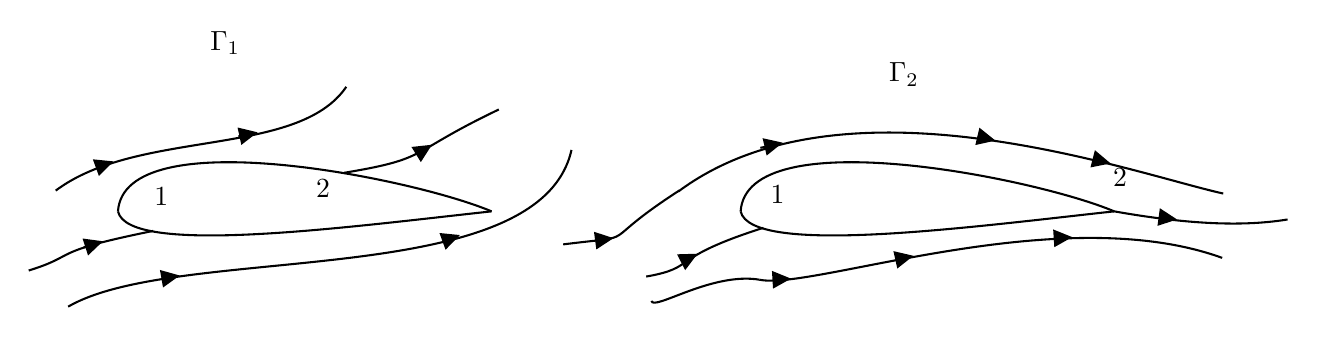
\begin{tikzpicture}[x=0.75pt,y=0.75pt,yscale=-1,xscale=1]
%uncomment if require: \path (0,285); %set diagram left start at 0, and has height of 285

%Curve Lines [id:da757474519234518] 
\draw    (40,120) .. controls (43.01,75.91) and (182.01,103.91) .. (220,120) ;
%Curve Lines [id:da5766387891735065] 
\draw    (40,120) .. controls (45.01,141.91) and (151.51,127.41) .. (220,120) ;
%Curve Lines [id:da7381550438058913] 
\draw    (340,120) .. controls (343.01,75.91) and (482.01,103.91) .. (520,120) ;
%Curve Lines [id:da8883065709307116] 
\draw    (340,120) .. controls (345.01,141.91) and (451.51,127.41) .. (520,120) ;
%Curve Lines [id:da7947732987676788] 
\draw    (10,110) .. controls (50,80) and (126.51,94.41) .. (150,60) ;
%Curve Lines [id:da7784136943432587] 
\draw    (-3,148.5) .. controls (21.51,140.91) and (5.52,139.83) .. (57.01,129.41) ;
%Curve Lines [id:da714986774675068] 
\draw    (16.01,165.91) .. controls (69.51,134.91) and (243.01,159.41) .. (258.51,90.41) ;
%Curve Lines [id:da7768122235559649] 
\draw    (149,101.41) .. controls (191.01,94.41) and (178.51,92.41) .. (223.51,70.91) ;
%Curve Lines [id:da34240417961624026] 
\draw    (294.51,151.41) .. controls (320.01,146.91) and (304.01,142.91) .. (351,127.91) ;
%Curve Lines [id:da0038959201144186384] 
\draw    (519.51,119.91) .. controls (550.51,125.41) and (579.01,127.91) .. (603.51,123.91) ;
%Curve Lines [id:da8381468549415312] 
\draw    (310.01,110.41) .. controls (390.01,50.91) and (529.51,101.91) .. (572.51,111.41) ;
%Curve Lines [id:da4264424078214477] 
\draw    (254.51,135.91) .. controls (294.51,130.91) and (268.01,137.41) .. (310.51,109.91) ;
%Curve Lines [id:da26038258191350194] 
\draw    (349.01,152.91) .. controls (374.01,158.41) and (493.51,113.91) .. (572.01,142.41) ;
%Curve Lines [id:da200973118006885] 
\draw    (297.01,163.16) .. controls (298.01,168.16) and (326.01,149.16) .. (349.01,152.91) ;
%Straight Lines [id:da5173954209160103] 
\draw    (29.51,98.91) -- (34.94,96.94) ;
\draw [shift={(37.76,95.91)}, rotate = 160.02] [fill={rgb, 255:red, 0; green, 0; blue, 0 }  ][line width=0.08]  [draw opacity=0] (8.93,-4.29) -- (0,0) -- (8.93,4.29) -- cycle    ;
%Straight Lines [id:da20555746266271058] 
\draw    (98.01,83.91) -- (104.33,82.55) ;
\draw [shift={(107.26,81.91)}, rotate = 167.8] [fill={rgb, 255:red, 0; green, 0; blue, 0 }  ][line width=0.08]  [draw opacity=0] (8.93,-4.29) -- (0,0) -- (8.93,4.29) -- cycle    ;
%Straight Lines [id:da18452635602009537] 
\draw    (23.51,137.41) -- (29.91,135.34) ;
\draw [shift={(32.76,134.41)}, rotate = 162.03] [fill={rgb, 255:red, 0; green, 0; blue, 0 }  ][line width=0.08]  [draw opacity=0] (8.93,-4.29) -- (0,0) -- (8.93,4.29) -- cycle    ;
%Straight Lines [id:da564713731614449] 
\draw    (61.26,152.41) -- (66.81,151.44) ;
\draw [shift={(69.76,150.91)}, rotate = 169.99] [fill={rgb, 255:red, 0; green, 0; blue, 0 }  ][line width=0.08]  [draw opacity=0] (8.93,-4.29) -- (0,0) -- (8.93,4.29) -- cycle    ;
%Straight Lines [id:da16892046108612524] 
\draw    (196.51,134.41) -- (201.94,132.44) ;
\draw [shift={(204.76,131.41)}, rotate = 160.02] [fill={rgb, 255:red, 0; green, 0; blue, 0 }  ][line width=0.08]  [draw opacity=0] (8.93,-4.29) -- (0,0) -- (8.93,4.29) -- cycle    ;
%Straight Lines [id:da23709222440505573] 
\draw    (184.01,92.41) -- (188.71,89.5) ;
\draw [shift={(191.26,87.91)}, rotate = 148.17] [fill={rgb, 255:red, 0; green, 0; blue, 0 }  ][line width=0.08]  [draw opacity=0] (8.93,-4.29) -- (0,0) -- (8.93,4.29) -- cycle    ;
%Straight Lines [id:da7801353976722618] 
\draw    (271.26,133.91) -- (275.79,133.31) ;
\draw [shift={(278.76,132.91)}, rotate = 172.41] [fill={rgb, 255:red, 0; green, 0; blue, 0 }  ][line width=0.08]  [draw opacity=0] (8.93,-4.29) -- (0,0) -- (8.93,4.29) -- cycle    ;
%Straight Lines [id:da5382263830192704] 
\draw    (349.51,89.41) -- (357.34,87.59) ;
\draw [shift={(360.26,86.91)}, rotate = 166.91] [fill={rgb, 255:red, 0; green, 0; blue, 0 }  ][line width=0.08]  [draw opacity=0] (8.93,-4.29) -- (0,0) -- (8.93,4.29) -- cycle    ;
%Straight Lines [id:da8597748721083103] 
\draw    (454.26,83.91) -- (459.84,85.23) ;
\draw [shift={(462.76,85.91)}, rotate = 193.24] [fill={rgb, 255:red, 0; green, 0; blue, 0 }  ][line width=0.08]  [draw opacity=0] (8.93,-4.29) -- (0,0) -- (8.93,4.29) -- cycle    ;
%Straight Lines [id:da24822087960525052] 
\draw    (510.51,94.91) -- (515.36,96.16) ;
\draw [shift={(518.26,96.91)}, rotate = 194.47] [fill={rgb, 255:red, 0; green, 0; blue, 0 }  ][line width=0.08]  [draw opacity=0] (8.93,-4.29) -- (0,0) -- (8.93,4.29) -- cycle    ;
%Straight Lines [id:da35895933983316564] 
\draw    (311.51,144.41) -- (316.6,141.79) ;
\draw [shift={(319.26,140.41)}, rotate = 152.7] [fill={rgb, 255:red, 0; green, 0; blue, 0 }  ][line width=0.08]  [draw opacity=0] (8.93,-4.29) -- (0,0) -- (8.93,4.29) -- cycle    ;
%Straight Lines [id:da8989308157600859] 
\draw    (356.01,152.91) -- (361.27,152.6) ;
\draw [shift={(364.26,152.41)}, rotate = 176.53] [fill={rgb, 255:red, 0; green, 0; blue, 0 }  ][line width=0.08]  [draw opacity=0] (8.93,-4.29) -- (0,0) -- (8.93,4.29) -- cycle    ;
%Straight Lines [id:da7471632193787989] 
\draw    (416.51,142.91) -- (420.33,142.06) ;
\draw [shift={(423.26,141.41)}, rotate = 167.47] [fill={rgb, 255:red, 0; green, 0; blue, 0 }  ][line width=0.08]  [draw opacity=0] (8.93,-4.29) -- (0,0) -- (8.93,4.29) -- cycle    ;
%Straight Lines [id:da8037532692120464] 
\draw    (492.01,132.91) -- (496.77,132.61) ;
\draw [shift={(499.76,132.41)}, rotate = 176.31] [fill={rgb, 255:red, 0; green, 0; blue, 0 }  ][line width=0.08]  [draw opacity=0] (8.93,-4.29) -- (0,0) -- (8.93,4.29) -- cycle    ;
%Straight Lines [id:da0934187170100993] 
\draw    (542.76,122.91) -- (547.29,123.52) ;
\draw [shift={(550.26,123.91)}, rotate = 187.59] [fill={rgb, 255:red, 0; green, 0; blue, 0 }  ][line width=0.08]  [draw opacity=0] (8.93,-4.29) -- (0,0) -- (8.93,4.29) -- cycle    ;

% Text Node
\draw (83,32) node [anchor=north west][inner sep=0.75pt]    {$\Gamma _{1}$};
% Text Node
\draw (410,47) node [anchor=north west][inner sep=0.75pt]    {$\Gamma _{2}$};
% Text Node
\draw (56,107) node [anchor=north west][inner sep=0.75pt]    {$1$};
% Text Node
\draw (134,103) node [anchor=north west][inner sep=0.75pt]    {$2$};
% Text Node
\draw (353,106) node [anchor=north west][inner sep=0.75pt]    {$1$};
% Text Node
\draw (518,98) node [anchor=north west][inner sep=0.75pt]    {$2$};


\end{tikzpicture}

  \caption{在势流中不同环量值流过翼型在给定攻角。1和2都是驻点}
  \label{fig:stag}
\end{figure}
展示了不同$\Gamma$的流动流过相同翼型在相同攻角的情况。
乍一看,似乎令人进退两难。从实验中,我们知道,给定翼型
在给定攻角的情况下,只会产生一个单值升力。所以,尽管有
无数种势流解,大自然知道如何去选取一种合适的解。显然,
在前述的解法讨论中,并不完全---我们需要一种条件去确定给
定翼型在给定攻角下的$\Gamma$。

为了找到这个条件,让我们先查看一些从静止的初始条件到运动
的绕翼型流动的发展实验情况。流动一开始,流动模式是从绕着
翼型开始发展的。在早期发展的时间,流动是绕着尖后缘点从下
翼面流到上翼面的,和图\ref{fig:stag}中左图相似。然而,更
准确的考虑无粘不可压流动表明,在尖后缘点的速度是无穷大的
。因此,这种流动是不能被大自然长时间容忍的。然而,真实的
流过翼型的流动,在上翼面的驻点会向后缘点移动。最后,在初
始瞬态过程结束后,稳定的流动状态就达到了,即{\color{noteorange}
气流是平滑的从后缘点离开上翼面和下翼面}。这种流动模式就
是图\ref{fig:stag}中的右图,并且表示了在翼型上稳定的流动
类型。

再次强调,给定翼型在给定攻角下建立稳定流动时,大自然会自
动自动产生一个满足要求的特定环量,这个环量使得气流平滑的
离开后缘点。这就是{\bfseries 库塔条件(Kutta condition)}。

为了使库塔条件理论化,我们需要更多的在后缘点的自然流动的
细节。后缘点处可以有一个有限的角度,或者可以是圆弧过渡的。
首先,考虑后缘点处是一个有限角度的情形。记上翼面和下翼面
的速度分别是$V_1$和$V_2$,如图\ref{fig:kutta},
\begin{figure}[!ht]
  \centering
  % ! TEX root = ./Incompressible_Flow_over_Airfoils.tex 

\tikzset{every picture/.style={line width=0.75pt}} %set default line width to 0.75pt        

\begin{tikzpicture}[x=0.75pt,y=0.75pt,yscale=-1,xscale=1]
%uncomment if require: \path (0,285); %set diagram left start at 0, and has height of 285

%Straight Lines [id:da09821137326284046] 
\draw    (110,100) -- (210,130) ;
%Straight Lines [id:da4215300487084799] 
\draw    (210,130) -- (110,160) ;
%Curve Lines [id:da27350478194701067] 
\draw    (110,100) .. controls (86.51,118.41) and (133.51,125.41) .. (110,160) ;
%Straight Lines [id:da5362893989420019] 
\draw    (110,100) -- (136.59,107.85) ;
\draw [shift={(138.51,108.41)}, rotate = 196.44] [color={rgb, 255:red, 0; green, 0; blue, 0 }  ][line width=0.75]    (10.93,-3.29) .. controls (6.95,-1.4) and (3.31,-0.3) .. (0,0) .. controls (3.31,0.3) and (6.95,1.4) .. (10.93,3.29)   ;
%Straight Lines [id:da8226716333160915] 
\draw    (110,99.5) -- (169.6,118.31) ;
\draw [shift={(171.51,118.91)}, rotate = 197.52] [color={rgb, 255:red, 0; green, 0; blue, 0 }  ][line width=0.75]    (10.93,-3.29) .. controls (6.95,-1.4) and (3.31,-0.3) .. (0,0) .. controls (3.31,0.3) and (6.95,1.4) .. (10.93,3.29)   ;
%Straight Lines [id:da8636864097351891] 
\draw    (110,160) -- (192.1,135.49) ;
\draw [shift={(194.01,134.91)}, rotate = 163.37] [color={rgb, 255:red, 0; green, 0; blue, 0 }  ][line width=0.75]    (10.93,-3.29) .. controls (6.95,-1.4) and (3.31,-0.3) .. (0,0) .. controls (3.31,0.3) and (6.95,1.4) .. (10.93,3.29)   ;
%Straight Lines [id:da05016986424572667] 
\draw    (110,160) -- (141.09,150.97) ;
\draw [shift={(143.01,150.41)}, rotate = 163.81] [color={rgb, 255:red, 0; green, 0; blue, 0 }  ][line width=0.75]    (10.93,-3.29) .. controls (6.95,-1.4) and (3.31,-0.3) .. (0,0) .. controls (3.31,0.3) and (6.95,1.4) .. (10.93,3.29)   ;
%Straight Lines [id:da8424011217264318] 
\draw    (110,100) -- (197.09,125.85) ;
\draw [shift={(199.01,126.41)}, rotate = 196.53] [color={rgb, 255:red, 0; green, 0; blue, 0 }  ][line width=0.75]    (10.93,-3.29) .. controls (6.95,-1.4) and (3.31,-0.3) .. (0,0) .. controls (3.31,0.3) and (6.95,1.4) .. (10.93,3.29)   ;
%Straight Lines [id:da6770379071467885] 
\draw    (110,160) -- (168.1,142.49) ;
\draw [shift={(170.01,141.91)}, rotate = 163.23] [color={rgb, 255:red, 0; green, 0; blue, 0 }  ][line width=0.75]    (10.93,-3.29) .. controls (6.95,-1.4) and (3.31,-0.3) .. (0,0) .. controls (3.31,0.3) and (6.95,1.4) .. (10.93,3.29)   ;
%Straight Lines [id:da08219164072740859] 
\draw  [dash pattern={on 4.5pt off 4.5pt}]  (210,130) -- (268.03,139.67) ;
\draw [shift={(270,140)}, rotate = 189.46] [color={rgb, 255:red, 0; green, 0; blue, 0 }  ][line width=0.75]    (10.93,-3.29) .. controls (6.95,-1.4) and (3.31,-0.3) .. (0,0) .. controls (3.31,0.3) and (6.95,1.4) .. (10.93,3.29)   ;
%Straight Lines [id:da8646964142450253] 
\draw  [dash pattern={on 4.5pt off 4.5pt}]  (210,130) -- (268.03,120.33) ;
\draw [shift={(270,120)}, rotate = 170.54] [color={rgb, 255:red, 0; green, 0; blue, 0 }  ][line width=0.75]    (10.93,-3.29) .. controls (6.95,-1.4) and (3.31,-0.3) .. (0,0) .. controls (3.31,0.3) and (6.95,1.4) .. (10.93,3.29)   ;
%Curve Lines [id:da44117033215025336] 
\draw    (380,90) .. controls (420,60) and (460.76,85.41) .. (480,110) ;
%Curve Lines [id:da08129815203793034] 
\draw    (380,120) .. controls (420,90) and (433.26,90.41) .. (480,120) ;
%Curve Lines [id:da34973148212289695] 
\draw    (480,110) .. controls (484.26,114.91) and (484.76,121.41) .. (480,120) ;
%Straight Lines [id:da14103967306792997] 
\draw  [dash pattern={on 4.5pt off 4.5pt}]  (480,110) -- (508.8,148.4) ;
\draw [shift={(510,150)}, rotate = 233.13] [color={rgb, 255:red, 0; green, 0; blue, 0 }  ][line width=0.75]    (10.93,-3.29) .. controls (6.95,-1.4) and (3.31,-0.3) .. (0,0) .. controls (3.31,0.3) and (6.95,1.4) .. (10.93,3.29)   ;
%Straight Lines [id:da8591768857204978] 
\draw  [dash pattern={on 4.5pt off 4.5pt}]  (480,120) -- (503.59,152.79) ;
\draw [shift={(504.76,154.41)}, rotate = 234.26] [color={rgb, 255:red, 0; green, 0; blue, 0 }  ][line width=0.75]    (10.93,-3.29) .. controls (6.95,-1.4) and (3.31,-0.3) .. (0,0) .. controls (3.31,0.3) and (6.95,1.4) .. (10.93,3.29)   ;

% Text Node
\draw (206,100) node [anchor=north west][inner sep=0.75pt]    {$a$};
% Text Node
\draw (226,139) node [anchor=north west][inner sep=0.75pt]    {$V_{1}$};
% Text Node
\draw (229,98) node [anchor=north west][inner sep=0.75pt]    {$V_{2}$};
% Text Node
\draw (496,109) node [anchor=north west][inner sep=0.75pt]    {$V_{1}$};
% Text Node
\draw (459,129) node [anchor=north west][inner sep=0.75pt]    {$V_{2}$};
% Text Node
\draw (479,90) node [anchor=north west][inner sep=0.75pt]    {$a$};
% Text Node
\draw (142,39) node [anchor=north west][inner sep=0.75pt]   [align=left] {有限角度};
% Text Node
\draw (426,39) node [anchor=north west][inner sep=0.75pt]   [align=left] {圆弧};
% Text Node
\draw (110,169) node [anchor=north west][inner sep=0.75pt]   [align=left] {$在点a\text{:}V_1=V_2=0$};
% Text Node
\draw (380,169) node [anchor=north west][inner sep=0.75pt]   [align=left] {$在点a\text{:}V1=V2\neq0$};


\end{tikzpicture}

  \caption{不同后缘点的形状和库塔条件的关系}
  \label{fig:kutta}
\end{figure}
$V_1$是在点$a$平行于上翼面的速度,$V_2$是在点$a$平行于下
翼面的速度。对于一个有限角度的后缘点,如果在点$a$的两个
速度都是有限的,那么我们在同一个点就有两个不同方向的两个速度
,如图\ref{fig:kutta}左图所示。但是,这是在物理上是不可能
的,唯一的办法就是让$V_1$和$V_2$都等于0 。也就是说,对于
有限角度的后缘点,$a$点就是驻点。相反的是,对于圆弧过渡的
后缘点,$V_1$和$V_2$在$a$点方向相同,并且$V_1$和$V_2$都是
有限值。但是,$a$点的压强是一个唯一的值,将伯努利方程
应用于上下翼面接近于$a$点处,得到
\[
  P_a+\frac{1}{2}\rho V_1^2=P_a+\frac{1}{2} \rho V_2^2
\]
或者
\[
  V_1=V_2
\]
因此,对于圆弧过渡的后缘点,我们可以发现,从翼型后缘点离开
上下翼面的速度是有限的,并且大小和方向都是相等的。

我们可以将库塔条件总结表述如下:
\begin{enumerate}
  \item 对于给定翼型在给定攻角的情况下,$\Gamma$的值要使得
    气流平滑地离开后缘点。
  \item 如果后缘角是有限的,那么后缘点就是一个驻点。
  \item 如果后缘角是圆弧过渡的,那么气流在后缘点离开上下翼面的
    速度大小是有限的,并且大小和方向都是一样的。
\end{enumerate}

再次考虑使用面涡模拟翼型的方法,面涡不论是放在翼面还是中弧线上。
沿着面涡的分布,面涡的强度都是变化的,并且记作$\gamma(s)$。库塔
条件使用面涡来表述如下。在后缘点(TE),我们有
\[
  \gamma(\mathrm{TE})=V_1-V_2
\]
然而,对于有限角度的后缘点,$V_1=V_2=0 $;因此,$\gamma(\mathrm{TE})=0 $。
对于圆弧过渡的后缘点,$V_1=V_2\neq 0 $;因此,$\gamma(\mathrm{TE})=0 $。
因此,库塔条件使用面涡表述就是
\begin{empheq}[box=\widefbox]{equation*}
  \gamma(\mathrm{TE})=0 
\end{empheq}

\subsection{没有摩擦能产生升力吗?}
在前面的讨论中,我们强调,浸没在空气中的翼型受到的气动力是
分布在翼型表面上的压强和剪切力的净综合效应。更重要的是,我
们注意到,翼型的升力主要是由于翼面上的压强分布,并且剪应力
对于升力基本上没有影响。这很容易知道是为什么。请看图\ref{fig:stag}
中翼型的形状。回想到压强作用在翼面的法线上,对于这些翼型,
法向的压力基本上是竖直的,也就是升力的方向。
与之相反的是,剪应力作用在翼面的切线方向,对于这些翼型,剪
应力主要是在水平方向,也就是阻力的方向。因此压力是产生升力
的主导者,剪应力对升力的影响可以忽略不记。这就是为什么升力
可以在失速前精准的被无粘理论预测出来,正如本章所讨论的那样。

然而,如果我们生活在一个完美地无粘世界中,翼型就不能产生升力。
事实上,摩擦的存在就是有升力的原因。这听起来很奇怪,甚至与
我们前一段的陈述相互矛盾。为什么会这样?答案就是,在真实生
活中,自然确保气流在后缘点平滑的离开的方法就是自然选择气流
的机制,即粘性边界层一直附着在翼型表面,直到后缘点。自然通
过摩擦来确保达到库塔条件。如果没有粘性边界层(如没有摩擦)
,在自然界中就没有物理机制可以满足库塔条件。

所以我们被代入了最为讽刺的境地,升力是有翼型表面的压强分布
产生的---一种无粘现象,不存在没有摩擦(无粘)的世界中。在
这方面,我们可以说没有摩擦就没有升力。然而,我们以上述讨论
的内容明智地这么说。

\section{开尔文环量定理和启动涡}
库塔条件描述了翼型绕流的环流是一个正值(顺时针为正)确保气
流能平滑的流过后缘点。问题是:这个环量是这么产生的?它是凭
空产生的,还是整个流场的环量都是守恒的呢?

如图\ref{fig:circulation},考虑任意一个无粘、不可压流动。
\begin{figure}[!ht]
  \centering
  % ! TEX root = ./Incompressible_Flow_over_Airfoils.tex

\tikzset{every picture/.style={line width=0.75pt}} %set default line width to 0.75pt        

\begin{tikzpicture}[x=0.75pt,y=0.75pt,yscale=-1,xscale=1]
%uncomment if require: \path (0,360); %set diagram left start at 0, and has height of 360

%Curve Lines [id:da6593875671900111] 
\draw    (110,120) .. controls (239.76,121.41) and (330,70) .. (370,40) ;
%Curve Lines [id:da5152113804444653] 
\draw    (110,180) .. controls (180.76,166.41) and (332.26,111.91) .. (410,120) ;
%Curve Lines [id:da811879248462616] 
\draw    (110,220) .. controls (182.76,209.91) and (376.76,175.41) .. (410,220) ;
%Straight Lines [id:da9503684630542251] 
\draw    (139,120) -- (140.78,119.78) ;
\draw [shift={(143.76,119.41)}, rotate = 172.98] [fill={rgb, 255:red, 0; green, 0; blue, 0 }  ][line width=0.08]  [draw opacity=0] (8.93,-4.29) -- (0,0) -- (8.93,4.29) -- cycle    ;
%Straight Lines [id:da5896891634358687] 
\draw    (190,113.91) -- (193.27,113.65) ;
\draw [shift={(196.26,113.41)}, rotate = 175.43] [fill={rgb, 255:red, 0; green, 0; blue, 0 }  ][line width=0.08]  [draw opacity=0] (8.93,-4.29) -- (0,0) -- (8.93,4.29) -- cycle    ;
%Straight Lines [id:da5521183292347811] 
\draw    (241.5,102.41) -- (244.36,101.67) ;
\draw [shift={(247.26,100.91)}, rotate = 165.41] [fill={rgb, 255:red, 0; green, 0; blue, 0 }  ][line width=0.08]  [draw opacity=0] (8.93,-4.29) -- (0,0) -- (8.93,4.29) -- cycle    ;
%Straight Lines [id:da046097384932481056] 
\draw    (295.76,82.91) -- (298.53,81.66) ;
\draw [shift={(301.26,80.41)}, rotate = 155.56] [fill={rgb, 255:red, 0; green, 0; blue, 0 }  ][line width=0.08]  [draw opacity=0] (8.93,-4.29) -- (0,0) -- (8.93,4.29) -- cycle    ;
%Straight Lines [id:da04541396429043876] 
\draw    (330.26,65.91) -- (332.69,64.46) ;
\draw [shift={(335.26,62.91)}, rotate = 149.04] [fill={rgb, 255:red, 0; green, 0; blue, 0 }  ][line width=0.08]  [draw opacity=0] (8.93,-4.29) -- (0,0) -- (8.93,4.29) -- cycle    ;
%Straight Lines [id:da7876927873324759] 
\draw    (139.76,173.41) -- (140.95,172.97) ;
\draw [shift={(143.76,171.91)}, rotate = 159.44] [fill={rgb, 255:red, 0; green, 0; blue, 0 }  ][line width=0.08]  [draw opacity=0] (8.93,-4.29) -- (0,0) -- (8.93,4.29) -- cycle    ;
%Straight Lines [id:da06331339935669789] 
\draw    (200.76,156.41) -- (203.8,155.91) ;
\draw [shift={(206.76,155.41)}, rotate = 170.54] [fill={rgb, 255:red, 0; green, 0; blue, 0 }  ][line width=0.08]  [draw opacity=0] (8.93,-4.29) -- (0,0) -- (8.93,4.29) -- cycle    ;
%Straight Lines [id:da10300319237850664] 
\draw    (250.26,143.91) -- (252.48,143.03) ;
\draw [shift={(255.26,141.91)}, rotate = 158.2] [fill={rgb, 255:red, 0; green, 0; blue, 0 }  ][line width=0.08]  [draw opacity=0] (8.93,-4.29) -- (0,0) -- (8.93,4.29) -- cycle    ;
%Straight Lines [id:da25013412556469916] 
\draw    (321.76,126.91) ;
\draw [shift={(323.76,126.41)}, rotate = 165.96] [fill={rgb, 255:red, 0; green, 0; blue, 0 }  ][line width=0.08]  [draw opacity=0] (8.93,-4.29) -- (0,0) -- (8.93,4.29) -- cycle    ;
%Straight Lines [id:da6407934074535004] 
\draw    (129.76,217.41) -- (130.78,217.29) ;
\draw [shift={(133.76,216.91)}, rotate = 172.87] [fill={rgb, 255:red, 0; green, 0; blue, 0 }  ][line width=0.08]  [draw opacity=0] (8.93,-4.29) -- (0,0) -- (8.93,4.29) -- cycle    ;
%Straight Lines [id:da4615476728563894] 
\draw    (191.76,208.41) -- (193.28,208.25) ;
\draw [shift={(196.26,207.91)}, rotate = 173.66] [fill={rgb, 255:red, 0; green, 0; blue, 0 }  ][line width=0.08]  [draw opacity=0] (8.93,-4.29) -- (0,0) -- (8.93,4.29) -- cycle    ;
%Straight Lines [id:da9779940169184937] 
\draw    (241.26,202.41) -- (241.79,202.34) ;
\draw [shift={(244.76,201.91)}, rotate = 171.87] [fill={rgb, 255:red, 0; green, 0; blue, 0 }  ][line width=0.08]  [draw opacity=0] (8.93,-4.29) -- (0,0) -- (8.93,4.29) -- cycle    ;
%Straight Lines [id:da9020973429401704] 
\draw    (299.26,197.91) ;
\draw [shift={(301.76,197.41)}, rotate = 168.69] [fill={rgb, 255:red, 0; green, 0; blue, 0 }  ][line width=0.08]  [draw opacity=0] (8.93,-4.29) -- (0,0) -- (8.93,4.29) -- cycle    ;
%Straight Lines [id:da43916377488014824] 
\draw    (357.26,199.41) -- (358.83,199.76) ;
\draw [shift={(361.76,200.41)}, rotate = 192.53] [fill={rgb, 255:red, 0; green, 0; blue, 0 }  ][line width=0.08]  [draw opacity=0] (8.93,-4.29) -- (0,0) -- (8.93,4.29) -- cycle    ;
%Curve Lines [id:da5222840687482979] 
\draw  [dash pattern={on 4.5pt off 4.5pt}]  (140,140) .. controls (180,110) and (216.26,121.5) .. (230,150) ;
%Curve Lines [id:da4165207301071254] 
\draw  [dash pattern={on 4.5pt off 4.5pt}]  (140,140) .. controls (82.76,201.41) and (254.76,227.41) .. (230,150) ;
%Curve Lines [id:da6047764522006289] 
\draw  [dash pattern={on 4.5pt off 4.5pt}]  (290,110) .. controls (330,80) and (397.26,106.41) .. (400,140) ;
%Curve Lines [id:da5317203333510179] 
\draw  [dash pattern={on 4.5pt off 4.5pt}]  (290,110) .. controls (243.76,164.41) and (398.76,213.41) .. (400,140) ;
%Straight Lines [id:da3514021396357123] 
\draw    (100,140) -- (140,140) ;
%Straight Lines [id:da25734728167981236] 
\draw    (400,140) -- (450,130) ;

% Text Node
\draw (79,132.4) node [anchor=north west][inner sep=0.75pt]    {$C_{1}$};
% Text Node
\draw (459,121.4) node [anchor=north west][inner sep=0.75pt]    {$C_{2}$};
% Text Node
\draw (191,42.4) node [anchor=north west][inner sep=0.75pt]    {$\Gamma _{1} =\Gamma _{2}$};
% Text Node
\draw (131,232) node [anchor=north west][inner sep=0.75pt]   [align=left] {流体微团在$t_1$\\时间沿着曲线$C_{1}$};
% Text Node
\draw (307,228) node [anchor=north west][inner sep=0.75pt]   [align=left] {相同的流体微团在\\一段时间后,即$t_2$\\时间,沿着不同的曲线$C_2$中};


\end{tikzpicture}

  \caption{开尔文定律}
  \label{fig:circulation}
\end{figure}
假设所有的彻体力都是0。选择任意一个闭合曲线$C_1$,这条曲线
确定了一定数量的在$t_1$时刻的流体单元。记沿着曲线$C_1$的环
量是$\Gamma_1=-\int _{C_1} \mathbf{V}\cdot \mathrm{d}\mathbf{s}$。
现在,让这些流体单元向下游流动,一段时间后,到达$t_2$时刻。
这些相同的流体单元将来自不同的曲线$C_2$,该曲线确定的环量
是$\Gamma_2=-\int _{C_2} \mathbf{V} \cdot \mathrm{d}\mathbf{s}$。
对于上述描述的状态,我们可以很容易地证明$\Gamma_1=\Gamma_2$。事实
上,我们追踪了一组特定的流体单元,我们可以描述为,由一组
连续的流体单元确定的闭合曲线,随着这些流体单元在全流场中
移动,这条闭合曲线确定的环量是一个常数。关于上述描述的数学
化表述可以简化为
\[
  \frac{\mathrm{D} \Gamma}{\mathrm{D} t}=0
\]
这就是说,有相同的流体单元组成的闭合曲线的环量对时间的变化率
是0。这就是{\bfseries 开尔文环量定理(Kelvin's circulation theoerm)}。
证明过程详见{\color{titleblue}附录\ref{kelvin theroem}}.
开尔文环量定理的一个有趣的结论就是,如果在某个瞬间,一个流动
表面是面涡,那么它将一直保持是面涡。

开尔文环量定理可以帮助解释绕翼型的环量是怎么产生的,如下。
考虑一个翼型在静止的流体中,如图\ref{fig:startvortex}
\begin{figure}[!ht]
  \centering
  % ! TEX root =./Incompressible_Flow_over_Airfoils.tex

\tikzset{every picture/.style={line width=0.75pt}} %set default line width to 0.75pt        

\begin{tikzpicture}[x=0.75pt,y=0.75pt,yscale=-1,xscale=1]
%uncomment if require: \path (0,360); %set diagram left start at 0, and has height of 360

%Shape: Polygon Curved [id:ds1411727865782737] 
\draw   (80,100) .. controls (68.51,32.41) and (201.49,15.59) .. (250,90) .. controls (298.51,164.41) and (269.51,172.41) .. (230,190) .. controls (190.49,207.59) and (161.49,199.59) .. (130,180) .. controls (98.51,160.41) and (91.49,167.59) .. (80,100) -- cycle ;
%Curve Lines [id:da6293293862133582] 
\draw    (120,90) .. controls (148.51,50.41) and (227.51,124.41) .. (240,150) ;
%Curve Lines [id:da44308727702954975] 
\draw    (120,90) .. controls (113.51,105.41) and (198.51,132.41) .. (240,150) ;
%Straight Lines [id:da18147270718988717] 
\draw    (50,60) -- (80,90) ;
%Curve Lines [id:da33190634449649714] 
\draw    (320,80) .. controls (340.76,-1.59) and (565.76,37.91) .. (590,120) ;
%Curve Lines [id:da4273091108123228] 
\draw    (320,80) .. controls (307.76,169.41) and (600.26,160.91) .. (590,120) ;
%Curve Lines [id:da01667939159590026] 
\draw    (350,80) .. controls (354.51,39.91) and (453.51,75.91) .. (460,100) ;
%Curve Lines [id:da44539055148167295] 
\draw    (350,80) .. controls (345.01,94.41) and (406.01,98.41) .. (460,100) ;
%Curve Lines [id:da3052696959417798] 
\draw  [dash pattern={on 4.5pt off 4.5pt}]  (460,100) .. controls (493.26,126.91) and (529.76,136.91) .. (560,130) ;
%Curve Lines [id:da17918828223900296] 
\draw  [dash pattern={on 4.5pt off 4.5pt}]  (540,120) .. controls (543.51,103.41) and (570.01,125.41) .. (560,130) ;
%Curve Lines [id:da6613061331627101] 
\draw    (500,50) .. controls (477.26,67.91) and (511.76,133.91) .. (480,150) ;
%Curve Lines [id:da9665395455277344] 
\draw    (360,60) .. controls (400.44,41.79) and (424.78,47.66) .. (448.55,68.69) ;
\draw [shift={(450,70)}, rotate = 222.34] [color={rgb, 255:red, 0; green, 0; blue, 0 }  ][line width=0.75]    (10.93,-3.29) .. controls (6.95,-1.4) and (3.31,-0.3) .. (0,0) .. controls (3.31,0.3) and (6.95,1.4) .. (10.93,3.29)   ;
%Curve Lines [id:da4858489509606265] 
\draw    (560,110) .. controls (559.03,96.69) and (553.73,85.37) .. (531.39,99.13) ;
\draw [shift={(530,100)}, rotate = 327.31] [color={rgb, 255:red, 0; green, 0; blue, 0 }  ][line width=0.75]    (10.93,-3.29) .. controls (6.95,-1.4) and (3.31,-0.3) .. (0,0) .. controls (3.31,0.3) and (6.95,1.4) .. (10.93,3.29)   ;
%Straight Lines [id:da5834417849984652] 
\draw    (550,120) -- (590,150) ;
%Straight Lines [id:da7932464552251242] 
\draw    (470,150) -- (480,180) ;
%Straight Lines [id:da6750477124024015] 
\draw    (490,150) -- (480,180) ;
%Straight Lines [id:da1468162505445323] 
\draw    (270,90) -- (308,90) ;
\draw [shift={(310,90)}, rotate = 180] [color={rgb, 255:red, 0; green, 0; blue, 0 }  ][line width=0.75]    (10.93,-3.29) .. controls (6.95,-1.4) and (3.31,-0.3) .. (0,0) .. controls (3.31,0.3) and (6.95,1.4) .. (10.93,3.29)   ;
%Straight Lines [id:da11718235105334185] 
\draw    (470,120) -- (490,140) ;
%Straight Lines [id:da4939225263931144] 
\draw    (470,120) -- (451.11,148.34) ;
\draw [shift={(450,150)}, rotate = 303.69] [color={rgb, 255:red, 0; green, 0; blue, 0 }  ][line width=0.75]    (10.93,-3.29) .. controls (6.95,-1.4) and (3.31,-0.3) .. (0,0) .. controls (3.31,0.3) and (6.95,1.4) .. (10.93,3.29)   ;
%Straight Lines [id:da6278616444384559] 
\draw    (490,140) -- (540,160) ;
%Straight Lines [id:da5845827423481111] 
\draw    (540,160) -- (501.94,150.49) ;
\draw [shift={(500,150)}, rotate = 14.04] [color={rgb, 255:red, 0; green, 0; blue, 0 }  ][line width=0.75]    (10.93,-3.29) .. controls (6.95,-1.4) and (3.31,-0.3) .. (0,0) .. controls (3.31,0.3) and (6.95,1.4) .. (10.93,3.29)   ;

% Text Node
\draw (141,92) node [anchor=north west][inner sep=0.75pt]   [align=left] {翼型};
% Text Node
\draw (16,113.4) node [anchor=north west][inner sep=0.75pt]    {$V=0$};
% Text Node
\draw (21,42.4) node [anchor=north west][inner sep=0.75pt]    {$C_{1}$};
% Text Node
\draw (221,12.4) node [anchor=north west][inner sep=0.75pt]    {$\Gamma _{1}$};
% Text Node
\draw (393,2.4) node [anchor=north west][inner sep=0.75pt]    {$\Gamma _{2} =\Gamma _{1} =0$};
% Text Node
\draw (506,22.4) node [anchor=north west][inner sep=0.75pt]    {$\Gamma _{3} =-\Gamma _{4}$};
% Text Node
\draw (478,52.4) node [anchor=north west][inner sep=0.75pt]    {$b$};
% Text Node
\draw (378,72) node [anchor=north west][inner sep=0.75pt]   [align=left] {翼型};
% Text Node
\draw (451,62.4) node [anchor=north west][inner sep=0.75pt]    {$\Gamma _{3}$};
% Text Node
\draw (521,72.4) node [anchor=north west][inner sep=0.75pt]    {$\Gamma _{4}$};
% Text Node
\draw (563,152) node [anchor=north west][inner sep=0.75pt]   [align=left] {启动涡};
% Text Node
\draw (469,181.4) node [anchor=north west][inner sep=0.75pt]    {$C_{2}$};
% Text Node
\draw (271,63.4) node [anchor=north west][inner sep=0.75pt]    {$V\infty $};
% Text Node
\draw (321,43.4) node [anchor=north west][inner sep=0.75pt]    {$a$};
% Text Node
\draw (598,112.4) node [anchor=north west][inner sep=0.75pt]    {$c$};
% Text Node
\draw (471,132.4) node [anchor=north west][inner sep=0.75pt]    {$d$};
% Text Node
\draw (441,111.4) node [anchor=north west][inner sep=0.75pt]    {$C_{3}$};
% Text Node
\draw (531,162.4) node [anchor=north west][inner sep=0.75pt]    {$C_{4}$};
% Text Node
\draw (83,212) node [anchor=north west][inner sep=0.75pt]   [align=left] {翼型周围的流体是静止的};
% Text Node
\draw (361,212.4) node [anchor=north west][inner sep=0.75pt]    {$流体开始流动后的某个瞬间$};


\end{tikzpicture}

  \caption{启动涡和绕翼型环量产生的原因}
  \label{fig:startvortex}
\end{figure}
中左图。因为全流场$\mathbf{V}=0$,所以闭合曲线$C_1$确定的
环量也是0 。现在开始让流体开始运动绕过翼型,气流将倾向于
在后缘周围卷起,如图\ref{fig:startvortex}中右图。这样的话,
后缘点的理论速度将达到无穷大。在真实生活中,这个速度将会是
一个非常大的有限的值。因此,在流动开始的最初时刻,
在后缘点的一个很薄的区域
一个非常大的速度梯度(也就是很大的涡强)就形成了。这个巨大
的涡强被相同的流体单元确定,因此当流体单元向下游流动时,
它被冲到下游。当它向下游运动时,这种薄的很大涡强的单元是
不稳定的,并且它将倾向于向前卷起,形成类似于点涡的图像。
这个涡就叫做{\bfseries 启动涡(starting vortex)},如图
\ref{fig:startvortex}右图所示。当翼型周围的气流达到稳定的
状态后,气流将平滑地流过后缘点(库塔条件),在后缘点
附近的很大的速度梯度也就消失了,在后缘点上也就不在产生涡强了。
然而,启动涡在流动开始流动的过程中已经产生了,并且随着流体
永远地稳定流向下游了。图\ref{fig:startvortex}中右图展示了
稳定流动后的流场,并且在下游某处出现涡流。一开始图\ref{fig:startvortex}
左图组成曲线$C_1$的流体单元流到下游,现在组成了曲线$C_2$,即
闭合曲线$abcda$,如图\ref{fig:startvortex}右图所示。
根据开尔文环量定理,绕曲线$C_2$(包含了翼型和后面的启动涡)
的环量和绕曲线$C_1$的环量是一样的,即都是0。所以
\[
  \Gamma_1=\Gamma_2=0 
\]
现在让我们将曲线$C_2$沿着曲线$bd$分成两个闭合的曲线,即
$C_3(bcdb)$和$C_4(abda)$。曲线$C_4$包围了启动涡,曲线
$C_3$包围了翼型。沿着$C_4$的环量$\Gamma_4$是因为启动涡的存在。
包围翼型的曲线$C_3$的环量是$\Gamma_4$。因为$bc$是曲线$C_3$
和$C_4$的公共边,所以$C_3$和$C_4$的环量之和就等于$C_2$的
环量,即
\[
  \Gamma_3+\Gamma_4=\Gamma_2
\]
然而,我们已经知道$\Gamma_2=0 $,所以
\[
  \Gamma_4=-\Gamma_3
\]
这就是说,绕机翼的环量等于绕启动涡环量的相反数。

这就引出了本节的关键和总结所在。当翼型绕流开始流动,
在尖后缘点处产生的很大的速度梯度产生一个很大的涡强,
这个涡强使得后缘点下游区域的气流卷起来,形成启动涡。
这个启动涡有一个逆时针的环量。因此,一个等大反向的
环量就在翼型上产生了。当这个开始流动过程就继续下去,
后缘点的涡强就不断流入启动涡,使得很大的逆时针环量
变得更大了。相应的,翼型上顺时针的环量也变得更大了,
使得流过后缘点的气流逐渐达到库塔条件,从而减弱了后
缘脱落涡的强度。最后,启动涡达到刚刚满足条件的强度,
使得等大反向的绕翼型的环量导致气流平滑地从后缘流出。
当这种情况发生,从后缘脱落涡的强度就变为了0 ,启动
涡的强度就不在增加了,绕翼型的环量将稳定存在。

\section{经典薄翼理论:对称翼型}
建立翼型的体坐标系,其中$x$沿弦线方向,$z$垂直于
弦线。

对于薄翼型,我们可以用沿中弧线分布的面涡代替这个翼型。
我们的目标是计算出在中弧线成为一条流线,并且满足库塔条件
下的$\gamma(s)$函数。一旦我们找到了一个特定的函数$\gamma(s)$
满足这两个条件,那么我们就可以用积分计算出总的环量,
然后用库塔--茹科夫斯基定理计算相应的升力。

考虑用一个沿中弧线分布的面涡取代翼型的情况。自由来流
的速度是$V_\infty$,翼型的攻角是$\alpha$。如果一个翼型
很薄,那么中弧线非常接近弦线,从很远的地方看,这个面涡
就是沿着弦线分布的。因此,再来一次替换,将沿中弧线的面涡
分布替换成沿弦线的分布,那么$\gamma=\gamma(x)$。我们
依然希望中弧线是流场中的一条流线,并且$\gamma(x)$被计算
出来后依然满足库塔条件,$\gamma(c)=0 $。这就是说,沿弦线
分布的面涡的强度决定了中弧线(不是弦线)是流线。

因为中弧线是流线,所以中弧线上所有点在垂直于中弧线上的
速度分量都是0 。流场中任何一点的速度就是远前方
自由来流的速度和面涡诱导出来的速度的矢量和。记$V_{\infty,n}$
是自由来流在中弧线法向的速度分量,$w'(s)$是由面涡
诱导出来的速度在中弧线法向上的速度分量。因此,因为中弧线
成为了一条流线,所以
\[
  V_{\infty,n}+w'(s)=0 
\]
在中弧线上任意一点都成立,这就是中弧线的边界条件。

对于一个小攻角的薄翼型,有
\[
  V_{\infty,n}=V_\infty(\alpha-\frac{\mathrm{d}z }{\mathrm{d}x})
\]
记$w(x)$是由面涡在弦线上一点诱导出来的速度在法向上的分量,由于
中弧线和弦线非常接近,那么可以做如下近似
\[
  w'(s)\approx w(x)
\]
我们希望计算出在坐标$x$的$w(x)$的值。考虑一个微元涡$\gamma \mathrm{d}\xi$
在沿着弦线距离原点$\xi$的地方。那么在$x$点由$\xi$产生的诱导速度
$\mathrm{d} w $就是
\[
  \mathrm{d} w=- \frac{\gamma(\xi) \mathrm{d} \xi}{2\pi(x-\xi)}
\]
相应的,在$x$点的速度就可以通过积分求解出来,即
\[
  w(x)=-\int _0^c \frac{\gamma (\xi)\mathrm{d}\xi}{2\pi(x-\xi)}
\]
将上面做的两个近似代入到中弧线的边界条件中就有
\[
  V_\infty(\alpha-\frac{\mathrm{d}z }{\mathrm{d}x})-\int _0^c \frac{\gamma(\xi)\mathrm{d}\xi}{2\pi(x-\xi)}=0
\]
或者
\[
  \frac{1}{2\pi}\int _0^c \frac{\gamma(\xi)\mathrm{d}\xi}{x-\xi}=V_\infty(\alpha-\frac{\mathrm{d} z }{\mathrm{d}x})
\]
这就是{\color{noteorange}薄翼理论的基本方程}。这描述了中弧线是流场中的
一条流线。

对于薄翼理论的基本方程,一个给定翼型在给定攻角下,$\alpha$和$\frac{\mathrm{d}z }{\mathrm{d}x}$
都是已知量。实际上,唯一的未知量就是$\gamma(\xi)$。基本方程是一个
积分方程,它的解$\gamma(\xi)$满足中弧线是流线的这个条件。薄翼理论
的核心问题是在满足中弧线是流线的条件下,找到满足库塔条件的解,即
$\gamma(c)=0 $。

如果是一个对称翼,那么
\[
  \frac{1}{2\pi}\int _0^c \frac{\gamma(\xi)\mathrm{d}\xi}{x-\xi}=V_\infty \alpha
\]
可以使用三角换元得到
\[
  \gamma(\theta)=2\alpha V_\infty \frac{1+\cos \theta}{\sin \theta}
\]
于是就有
\[
  \begin{split}
    \frac{1}{2\pi}\int _0^c \frac{\gamma(\theta)\sin  \theta \mathrm{d}\theta}{\cos \theta -\cos \theta_0}
    &=\frac{V_\infty \alpha}{\pi}\int _0^c \frac{(1+\cos \theta)\mathrm{d}\theta}{\cos \theta -\cos \theta_0}\\ 
    &=V_\infty \alpha
  \end{split}
\]
在后缘点处,$\theta=\pi$,那么有
\[
  \gamma(\pi)=2\alpha V_\infty \left.\frac{1+\cos \theta}{\sin \theta}\right| _{\theta=\pi}=
    2\alpha V_\infty \frac{0}{0}
\]
这是一个不确定的极限,使用洛必达法则得到
\[
  \gamma(\pi)=2\alpha V_\infty \frac{-\sin \pi}{\cos \pi}=0 
\]
满足库塔条件。

在这种情况下,现在求解升力系数。绕翼型的总环量是
\[
  \Gamma=\int _0 ^c \gamma(\xi)\mathrm{d}\xi 
\]
使用$\xi=\frac{c}{2 }(1-\cos \theta)$换元得到
\[
  \Gamma=\frac{c}{2}\int _0^\pi \gamma(\theta)\sin \theta \mathrm{d} \theta
\]
将$\gamma(\theta)$代入就可以得到
\[
  \Gamma=\alpha c V_\infty \int_0^\pi (1+\cos \theta)\mathrm{d}\theta =\pi \alpha c V_\infty 
\]
因此单位翼展上的升力就是
\[
  L'=\rho _\infty V_\infty \Gamma =\pi \alpha c V_\infty^2 
\]
因此升力系数就是,其中$S=c(1)$,
\[
  c_l=\frac{L'}{q_\infty S}
\]
得到
\[
  c_l=\frac{L'}{\frac{1}{2}\rho_\infty V_\infty^2 c(1)}=2\pi \alpha
\]
也就是说
\[
  升力曲线的斜率=\frac{\mathrm{d}c_l}{\mathrm{d}\alpha}=2\pi
\]
这是一个重要的结果,它表明了升力系数和攻角是线性相关的。同样,这依然
表明升力曲线的斜率等于$2\pi \,\,\mathrm{rad}^{-1}$。

根据前缘力矩计算公式
\[
  M'_{\mathrm{LE}}=-\int _0^c \xi (\mathrm{d}L)=
  -\rho_\infty V_\infty \int _0^c \xi \gamma(\xi)\mathrm{d}\xi
\]
作积分变换$\xi=\frac{c}{2}(1-\cos \theta)$代入$\gamma(\theta)$
积分得到
\[
  M'_{LE}=-q_\infty c^2 \frac{\pi \alpha}{2}
\]
所以前缘力矩系数就是
\[
  c_{m,le}=\frac{M'_{LE}}{q_\infty S c}
\]
其中,$S=c(1)$,所以前缘力矩系数就是
\[
  c_{m,le}=-\frac{\pi \alpha}{2}
\]
又
\[
  2\pi \alpha =c_l
\]
所以
\[
  c_{m,le}=\frac{c_l}{4}
\]
四分之一弦线处力矩的计算公式是
\[
  c_{m,\frac{c}{4}}=c_{m,le}+\frac{c_l}{4}
\]
所以$\frac{c}{4}$弦线处的力矩即
\[
  c_{m,\frac{c}{4}}=0
\]
这表明了{\color{noteorange}对称翼型的压心在$\frac{c}{4}$弦线处}。由
空气动力学中心的定义,我们得到
{\color{noteorange}对称翼型的气动中心和压心重合,都在$\frac{c}{4}$弦线处}。
\begin{notice}
压心的定义是对压心取矩为0,也就是压心处的气动力矩为0 。

空气动力中心(气动中心)的定义是翼型上存在一点使得对该点
取矩,气动力矩的大小和攻角的变化无关。

注意,当翼型的攻角变大时,压心要往前移,也就是说压心的位置和
攻角大小有关。所以,一般情况下,压心和气动中心不重合。

这里压心和气动中心重合的原因是,首先对$\frac{1}{4 }$弦线
处取力矩为0,所以就是压心。其次,这个力矩恒为0,和攻角
无关,所以就成为了气动中心。
\end{notice}

对本节内容做一个总结如下,对于对称翼型:
\begin{enumerate}
  \item $c_l=2\pi \alpha$ 
  \item 升力曲线的斜率是$2\pi$
  \item 压心和气动中心是重合的,也就是都在$\frac{c}{4}$弦线处
\end{enumerate}
\begin{example}
  考虑一种平盘在攻角$5^\circ$的情况下,计算1)升力系数;2)计算
  前缘力矩系数;3)关于$\frac{c}{4}$弦线处的力矩系数;4)关于
  后缘点的力矩系数;

  \[
    c_l=2 \pi \alpha=\frac{2\pi\times 5}{57.3}=0.5485
  \]
\[
c_{m,le}=- \frac{c_l}{4}=-0.137
\]
\[
  c_{m,\frac{c}{4}}=0
\]
\[
  c_{m,te}=\frac{3}{4}c_l=0.411
\]
\end{example}

对于弧形翼(有弯度的翼型)来说,$\frac{\mathrm{d}z }{\mathrm{d}x}$
不等于0,上述结论就不在适用了。与对称薄翼型一样,中弧线也是流场
中的一条流线,同样满足库塔条件。

同样,基本方程是
\[
  \frac{1}{2\pi}\int _0^c \frac{\gamma(\xi)\mathrm{d}\xi}{x-\xi}=V_\infty (\alpha-\frac{\mathrm{d}z }{\mathrm{d}x})
\]
换元$\xi=\frac{c}{2 }(1-\cos \theta)$,得到
\[
  \frac{1}{2\pi}\int _0^\pi \frac{\gamma(\theta)\sin \theta\mathrm{d}\theta}{\cos \theta -\cos \theta_0}
  =V_\infty \left(\alpha-\frac{\mathrm{d}z }{\mathrm{d}x}\right)
\]
将$\gamma(\theta)$展开成傅里叶正弦级数,即:
\[
  \gamma(\theta)=2V_\infty\left(A_0 \frac{1+\cos \theta}{\sin \theta}+
\sum _{n=1}^\infty A_n \sin n \theta\right)
\]
代入到基本方程中得到
\[
  \frac{1}{\pi}\int _0^\pi \frac{A_0\left(1+\cos \theta\right)\mathrm{d}\theta}{\cos \theta-\cos \theta_0}+
  \frac{1}{\pi}\sum_{n=1}^\infty \int _0^\pi \frac{A_n \sin n \theta \, \mathrm{d}\theta}{\cos \theta-\cos \theta_0}
  =\alpha -\frac{\mathrm{d}z }{\mathrm{d}x}
\]
使用积分结果(见{\color{titleblue}附录\ref{三角函数定积分}}),即:
\[
  \int_0^\pi \frac{\sin n \theta \sin \theta \, \mathrm{d}\theta}{\cos \theta -\cos \theta_0}
  =-\pi \cos n \theta_0
\]
和
\[
  \int _0^\pi \frac{1+\cos \theta}{\cos \theta -\cos \theta_0}\mathrm{d} \theta =\pi
\]
得到
\[
  A_0-\sum _{n=1}^\infty A_n \cos n \theta_0 =\alpha -\frac{\mathrm{d}z }{\mathrm{d} x}
\]
或者
\[
  \frac{\mathrm{d} z }{\mathrm{d}x }=\left(\alpha-A_0\right)+\sum_{n=1}^\infty A_n \cos n \theta_0
\]
上式可以在给定点$x$计算出来,这里$\frac{\mathrm{d}z }{\mathrm{d}x }$和$\theta_0$都是
和弦线上$x$点相关的参数,其中,$x=\frac{c}{2 }(1-\cos \theta_0)$。

回到上面的那个方程,这是将函数$\frac{\mathrm{d}z }{\mathrm{d}x}$用
傅里叶余弦级数展开的。那么函数$f(\theta)$可以用级数来表示
\[
  f(\theta)=B_0+\sum_{n=1}^\infty \cos n \theta
\]
其中,$0\leq \theta \geq \pi$。系数可以用如下的方法计算出来:
\[
  B_0=\frac{1}{\pi} \int _0^\pi f(\theta) \, \mathrm{d} \theta
\]
和
\[
  B_n=\frac{2}{\pi}\int _0 ^\pi f(\theta)\cos n \theta\, \mathrm{d} \theta
\]
$\frac{\mathrm{d} z }{\mathrm{d} x}$和$f(\theta)$是一样的,所以
\[
  \alpha-A_0=\frac{1}{\pi}\int _0^\pi \frac{\mathrm{d}z }{\mathrm{d}x }\, \mathrm{d} \theta_0
\]
和
\[
  A_n=\frac{2}{\pi}\int _0 ^\pi \frac{\mathrm{d} z }{\mathrm{d}x}\cos n \theta_0\,
  \mathrm{d} \theta_0
\]
请记住,$\frac{\mathrm{d}z }{\mathrm{d}x}$是关于$\theta_0$的函数。
从上面的方程可以看出,$A_0$与飞行迎角和中弧线的形状有关系,但是$A_n$
只和中弧线的形状有关。

在上面的讨论中,我们考虑了
气流流过一个有弯度的翼型在给定的形状$\frac{\mathrm{d}z }{\mathrm{d}x}$
和给定的攻角。为了使得中弧线成为流线,我们需要计算出沿弦线的面涡强度分布。
同样,也要满足库塔条件。$A_0$和$A_n$的实际数值可以在给定攻角下通过简单
的积分计算得到。当$\mathrm{d}z / \mathrm{d}x =0$的时候,那就是一个对称
翼型,是上述积分计算公式的一种特殊情况。

下面我们计算对于一个有弯度的翼型的空气动力系数。从前缘点到后缘点的
总环量可以通过下面的积分得到
\[
  \Gamma=\int _0^c \gamma(\xi)\,\mathrm{d}\xi =
  \int _0^\pi \gamma(\theta)\, \mathrm{d}\theta
\]
将我们得到的$\gamma(\theta)$代入到上式得到
\[
  \Gamma=c V_\infty \left[A_0\int _0^\pi \left(1+\cos \theta\right)\,\mathrm{d}\theta
+\sum _{n=1}^\infty A_n\int _0^\pi \sin n \theta \sin \theta \,\mathrm{d}\theta\right]
\]
其中
\[
  \int _0^\pi (1+\cos \theta)\, \mathrm{d} \theta=\pi
\]
\[
  \int _0^\pi \sin n \theta \sin \theta \,\mathrm{d}\theta =
  \begin{cases}
    \frac{\pi}{2 }&,n=1 \\ 
    0 &,n\neq 1
  \end{cases}
\]
因此,总环量就是
\[
  \Gamma=c V_\infty \left(\pi A_0 +\frac{\pi}{2 }A_1\right)
\]
根据库塔--茹科夫斯基定理得到单位翼展上的升力
\[
  L'=\rho_\infty V_\infty \Gamma=
  \rho_\infty V_\infty^2 c\left(\pi A_0+\frac{\pi}{2 }A_1\right)
\]
那么升力系数就是
\[
  c_l=\frac{L'}{\frac{1}{2 }\rho_\infty V_\infty ^2 c(1)}=\pi(2A_0+A_1)
\]
代入$A_0$和$A_1$的计算公式得到
\[
  c_l=2\pi \left[\alpha+\frac{1}{\pi}\int _0^\pi \frac{\mathrm{d}z }{\mathrm{d}x}(\cos \theta_0-1)
  \, \mathrm{d}\theta_0\right]
\]
也就是
\begin{empheq}[box=\widefbox]{equation*}
  升力线斜率=\frac{\mathrm{d}c_l }{\mathrm{d}\alpha}=2\pi
\end{empheq}
记住这是一个重要结果,对于对称翼型和有弯度的翼型升力线斜率都是$2\pi$。
事实上,这个从薄翼理论得到的结果对于所有翼型都适用,也就是所有
翼型的升力线斜率都是$2\pi$。请注意,对称翼型的升力系数$c_l$和有
弯度的翼型的升力系数是有区别的。回忆零升攻角$\alpha_{L=0}$的概念,
它一般是一个负值,升力线的方程可以写成
\[
  c_l=\frac{\mathrm{d}c_l}{\mathrm{d}\alpha}(\alpha-\alpha_{L=0})
\]
也即是 
\[
  c_l=2\pi(\alpha-\alpha_{L=0})
\]
比较我们推导的升力线方程,可以得到
\[
  \alpha_{L=0}=-\frac{1}{\pi}\int _0^\pi \frac{\mathrm{d}z }{\mathrm{d}\alpha}
  (\cos \theta_0-1)\,\mathrm{d}\theta_0
\]
这个方程提供了一种方法去预测零升攻角的大小。对于对称翼型的零升攻角就是0 。
相应的,对于弯度比较大的翼型,它的零升攻角的值就要大一些。

根据前缘力矩的定义
\[
  M'_{\mathrm{LE}}=-\int _0^c \xi (\mathrm{d}L)=
  -\rho_\infty V_\infty \int _0^c \xi \gamma(\xi)\mathrm{d}\xi
\]
换元,并将$\gamma(\theta)$代入,计算得到
\[
  c_{m,le}=-\frac{\pi}{2 }\left(A_0+A_1-\frac{A_2}{2}\right)
\]
将升力系数代入得到
\[
  c_{m,le}=-\left[\frac{c_l}{4}+\frac{\pi}{4}(A_1-A_2)\right]
\]
当$\mathrm{d}z /\mathrm{d}x=0$,即$A_1=A_2=0 $,代入到上式
就得到了对称翼型的前缘力矩。

$\frac{c}{4}$处的力矩可以通过
\[
  c_{m,\frac{c}{4}}=c_{m,le}+\frac{c_l}{4}
\]
计算得到
所以
\[
  c_{m,\frac{c}{4}}=-\frac{\pi}{4}\left(A_1-A_2\right)
\]
不像对称翼型那样,有弯度的翼型$\frac{c}{4}$处的力矩不等于0 。
上式表明,四分之一弦线处的力矩是有限的。然而$A_1$和$A_2$是
只和翼型的弯度大小有关的,而与攻角大小无关。所以
四分之一弦线处是有弯度翼型的理论的气动中心。

压心的位置可以通过下面的公式计算得到
\[
  x_{cp}=-\frac{M'_{LE}}{L'}=-\frac{c_{m,le}c}{L'}
\]
也就是
\[
  x_{cp}=\frac{c}{4}\left[1+\frac{\pi}{c_l}\left(A_1-A_2\right)\right]
\]
这表明有弯度翼型的压心位置是随着升力系数的大小变化而变化的。
因此,攻角变化,压心也随着变化。事实上,当升力趋向于0,
$x_{cp}$就移动到无穷远处了;这就是说,它离开了翼型。因为
这样,压心并不是一个很方便的点来描述翼型上的力系。反而,
气动中心就十分方便来描述翼型上的力系和力矩系。

\begin{example}
  给定翼型NACA 23012 。这个翼型的中弧线方程是
  \[
    \frac{z}{c}=2.6595\left[\left(\frac{x}{c}\right)^3 -0.6075
    \left(\frac{x}{c}\right)^2 +0.1147\left(\frac{x}{c}\right) 
  \right] \qquad 0\leq \frac{x}{c} \geq 0.2025 
  \]
  和
  \[
    \frac{z}{c}=0.02208\left(1-\frac{x}{c}\right) \qquad 0.2025 \leq \frac{x}{c} \geq 1.0 
  \]

计算a)零升攻角;b)$\alpha=4^\circ$时的升力系数;c)四分之一
弦线处的气动力矩系数;d)$\alpha=4^\circ$时的压心的位置,用$x_{cp} / c $表示。

首先,我们需要计算出$\frac{\mathrm{d}z }{\mathrm{d} x}$。对于给定的中弧线,有
\[
  \frac{\mathrm{d}z }{\mathrm{d}x}=2.6595
  \left[3\left(\frac{x}{c}\right)-1.215\left(\frac{x}{c}\right)+0.1147\right]
  \qquad 0 \leq \frac{x}{c} \geq 0.2025
\]
和
\[
  \frac{\mathrm{d}z }{\mathrm{d}x}=0.02208 \qquad 0.2025 \leq \frac{x}{c} \geq 1.0
\]
将坐标$x$变换到$\theta$,即$x=\frac{c}{2}(1-\cos \theta)$,我们有
\[
  \begin{split}
    \frac{\mathrm{d}z }{\mathrm{d}x}&=2.6595
  \left[\frac{3}{4}(1-2\cos \theta +\cos ^2 \theta)-0.6075(1-\cos \theta)+0.1147\right] \\ 
                                    &=
                                    0.6840-2.3736 \cos \theta +1.995 \cos ^2 \theta
                                    \qquad  0 \leq \theta \geq 0.9335 \,\,\mathrm{rad}
  \end{split}
\]
和
\[
  \frac{\mathrm{d}z }{\mathrm{d} x}=-0.02208 \qquad 0.9335 \leq \theta \geq \pi
\]
(a)
\[
  \alpha_{L=0}=\int _0^\pi \frac{\mathrm{d}z }{\mathrm{d}x}(\cos \theta-1)\,\mathrm{d}\theta=
  -0.0191\,\, \mathrm{rad}
\]
(b)
$\alpha=4^\circ=0.0698 \,\,\mathrm{rad}$,
\[
  c_l=2\pi (\alpha-\alpha_{L=0})=2\pi(0.0698+0.0191)=0.559
\]
(c)
我们需要先计算出$A_1$和$A_2$的值。
\[
  A_1=\frac{2}{\pi}\int _0^\pi \frac{\mathrm{d}z }{\mathrm{d}x }\cos \theta\,\mathrm{d} \theta
  =0.0954
\]
\[
  A_2=\frac{2}{\pi}\int _0^\pi \frac{\mathrm{d}z }{\mathrm{d}x} \cos 2 \theta\, \mathrm{d} \theta
  =0.0792
\]
于是
\[
  c_{m,\frac{c}{4}}=\frac{\pi}{4}(A_2-A_1)=\frac{\pi}{4}(0.0792-0.0954)=-0.0127
\]
(d)
由
\[
  x_{cp}=\frac{c}{4}\left[1+\frac{\pi}{c_l}\left(A_1-A_2\right)\right]
\]
于是
\[ 
  \begin{split}
    \frac{x_{cp}}{c}&=\frac{1}{4}\left[1+\frac{\pi}{c_l}\left(A_1-A_2\right)\right]\\
                    &=\frac{1}{4}\left[1+\frac{\pi}{0.559}(0.0954-0.0792)\right]=0.273
  \end{split}
\]
\end{example}

至此,本节的任务已经全部完成了。本节内容我们计算了薄翼型的升力系数,力矩系数
和前缘力矩等,还证明了升力线的斜率是$2\pi$。


